\documentclass{article}
\usepackage[letterpaper,top=2cm,bottom=2.5cm,left=3cm,right=3cm,marginparwidth=1.75cm]{geometry}
\usepackage[round]{natbib}
\usepackage{amsmath,amssymb,amsfonts}%
\usepackage{geometry}%
\usepackage{color}
\usepackage{graphicx}
\usepackage{authblk}
\usepackage{nameref}
\usepackage[right]{lineno}
\usepackage{subcaption}
\usepackage{tikz}
\usetikzlibrary{math,calc,positioning}
\usepackage{url}
\usepackage[symbol]{footmisc}
% JK: turning this off for the moment as I keep clicking through on links
% to the bibliography while reading the text and it's intensely annoying.
% Can reinstate when we're ready to preprint
% \usepackage[hidelinks]{hyperref}

\newcommand{\noderef}[1]{\textsf{#1}}
\newcommand{\tsinfer}[0]{\texttt{tsinfer}}
\newcommand{\kwarg}[0]{\texttt{KwARG}}
\newcommand{\argweaver}[0]{\texttt{ARGweaver}}
\newcommand{\relate}[0]{\texttt{Relate}}
\newcommand{\espalier}[0]{\texttt{Espalier}}

\begin{document}


\title{\vspace{-1.5em} \bf
A general and efficient representation of ancestral recombination graphs}

\author[1]{Yan~Wong}
\author[2,3$\star$]{Anastasia~Ignatieva}
\author[4,5$\star$]{Jere~Koskela}
\author[6]{Gregor~Gorjanc}
\author[7,8]{Anthony~W.~Wohns}
\author[1$\dagger$]{Jerome~Kelleher}
\affil[ ]{\mbox{}\vspace{-2.5em}}

\maketitle

\setlength{\skip\footins}{1em}
\setlength{\footnotemargin}{0.5em}
\renewcommand{\thefootnote}{\arabic{footnote}}
\footnotetext[1]{Big Data Institute, Li Ka Shing Centre for Health
Information and Discovery, University of Oxford, UK}
\footnotetext[2]{School of Mathematics and Statistics, University of Glasgow, UK}
\footnotetext[3]{Department of Statistics, University of Oxford, UK}
\footnotetext[4]{School of Mathematics, Statistics and Physics, Newcastle University, UK}
\footnotetext[5]{Department of Statistics, University of Warwick, UK}
\footnotetext[6]{The Roslin Institute and Royal (Dick) School of Veterinary Studies, University of Edinburgh, UK}
\footnotetext[7]{Broad Institute of MIT and Harvard, Cambridge, USA}
\footnotetext[8]{Department of Genetics, Stanford University School of Medicine, Stanford, USA}
\renewcommand{\thefootnote}{\fnsymbol{footnote}}
\footnotetext[1]{Joint second author, listed alphabetically}
\footnotetext[2]{Correspondence: jerome.kelleher@bdi.ox.ac.uk}

\vspace{-1em}

\begin{abstract}
New developments have made it possible to infer genetic genealogies in
the presence of recombination at scale, enabling many
downstream applications in population and statistical genetics.
The structure representing such recombinant genetic ancestry
is usually referred to as an ancestral recombination graph (ARG),
although there is some confusion about the interpretation and little
agreement on specific details.
We propose a concrete definition of ARGs
in terms of genomes and their intervals of genetic inheritance (gARG)
and contrast this with the classical event-based definition (eARG).
We show that eARGs are limited in the patterns
of genetic inheritance that can be represented,
and require a precise description of the details of all recombination events.
We show, in contrast, that the gARG definition
can fully capture the richness of modern large-scale datasets,
enables fine-grained
levels of precision about recombination to be represented,
and forms the basis of an efficient computational framework.
\end{abstract}

\textbf{Keywords:} Ancestral recombination graphs

\linenumbers
\section{Introduction}
\label{sec-intro}
Estimating the genetic genealogy of a set of genome sequences
under the influence of recombination,
usually known as an Ancestral Recombination Graph (ARG), is a long-standing
goal in genetics.
Broadly speaking, an ARG describes the different paths of genetic inheritance
caused by recombination, and encodes a sequence of correlated genealogical
trees along the genome.
Recent breakthroughs
in large-scale inference
methods~\citep{rasmussen2014genome,kelleher2019inferring,speidel2019method,
schaefer2021ancestral,wohns2022unified,zhang2023biobank,zhan2023towards}
and data representation~\citep{kelleher2016efficient,kelleher2018efficient}
have raised the realistic prospect of ARG-based analysis becoming a standard part
of the population and statistical genetics toolkit~\citep{hejase2020summary}.
Applications using inferred ARGs as input have begun to
appear~\citep{osmond2021estimating,fan2022genealogical,hejase2022deep,zhang2023biobank,
nowbandegani2023extremely,ignatieva2023distribution}
and many more are sure to
follow~\citep{harris2019database,harris2023using}.
See \citet{lewanski2023era} for a biologically oriented introduction to ARGs.

% TODO need to mention ARG-as-a-data-structure to clarify.
% What is the problem?
Although it is widely accepted that ARGs are important, there is significant
confusion about what, precisely, an ARG \emph{is}.
Originally, ARGs were defined by Griffiths and colleagues as an alternative
formulation of the coalescent with recombination~\citep{hudson1983properties},
where the stochastic process of coalescence and recombination
among ancestral lineages is formalised as a
% Note: please don't add "mathematical graph". If a reader doesn't know what a
% graph is they're not going to understand this paper.
graph~\citep{griffiths1991two,ethier1990two,griffiths1996ancestral,griffiths1997ancestral}.
Subsequently, an ARG  has come to be thought of as a data
structure~\citep{minichiello2006mapping}, i.e.\ describing
the outcome of such a stochastic process or a
genetic genealogy inferred from a sample of genome sequences.
However, the distinction between process and data structure is not clear cut
and subfields use the term
differently (see Appendix~\ref{sec-arg-history}).

% JK: this para need a major update, it's quite weak right now.
The word ``ARG'' is now widely used to refer to genetic genealogies in
general~\citep[e.g.][]{mathieson2020ancestry,hejase2020summary,
schaefer2021ancestral,harris2023using,zhang2023biobank},
encompassing the varied outputs from modern simulation and
inference methods~\citep{rasmussen2014genome, palamara2016argon, haller2018tree,
kelleher2019inferring, speidel2019method, baumdicker2021efficient, zhang2023biobank}.
This broad usage means there is a lack of consensus on the
exact object being defined, which causes problems, for example,
when evaluating inferred ARGs, and even when defining
what the criteria for success should be.
It also means there is no shared format for interchanging ARG data between
programs, resulting in the assorted negative consequences with which
geneticists are only too familiar~\citep{excoffier2006computer,gower2022demes}.
Perhaps most importantly, definitions linked to
the original stochastic process lead to an
overly narrow interpretation of ARGs, which is significantly
out of step with modern methods and large-scale datasets, and
can lead to missed opportunities in their application and usage.
Such problems go much deeper than pedantic discussion over terminology;
they directly inform what we should be attempting to estimate, how we
assess success, and the expected limitations on the precision
and accuracy of our inferences.
% Thanks for the phrase Gideon and Alex!
If not addressed, these problems will
impede progress in applying genetic genealogies to understand the biological world.

% Evidence of confusion to cite above in "problem" para?
% https://github.com/tskit-dev/what-is-an-arg-paper/issues/334
% The output of these programs is certainly not a collection of
% \emph{unrelated} local trees, as implied by,
% e.g.,
% \citet{hejase2020summary} when they state that \tsinfer\
% ``does not explicitly infer an ARG but rather a sequence of local
% gene trees''.
% More cites? Not worth harping on about now?
% https://github.com/tskit-dev/what-is-an-arg-paper/issues/38

% What do we do?
In this paper, we attempt to address these problems by
providing a precise definition of an ARG that is general enough to encompass
the output of popular simulation and inference methods.
We propose a definition of genetic genealogy in terms of specific genomes
and their intervals of genetic inheritance, and refer to this as
a ``genome ARG'', or ``gARG''.
This contrasts with the classical Griffiths approach,
based on recording evolutionary events, which we call
an ``event ARG'', or ``eARG''.
We show that the gARG encoding has a range of advantages over the
eARG approach, being flexible, efficient and, in particular,
allowing us to systematically encode uncertainty about
the precise details of recombination events.

% TODO: Provide a map of the paper's sections and how they tie together in support of gARG as a way forward.
% Here is a rough draft - it would be good to state the most important message (in one sentence or so) from each of the sections to help with frontloading key messages
% Genome ARGs &
% Event ARGs
In the following, we define the genome ARG (gARG) and contrast it with the event ARGs (eARG).
% Retrospective vs prospective
% TODO: This needs revision - see also https://github.com/tskit-dev/what-is-an-arg-paper/pull/380
We continue with a description of the usually held retrospective view of ARGs,
but note that ARGs can also be viewed as prospective, particularly in forwards-time
simulations. In the context of forwards-time simulations, we mention the
simplification operation, which removes ancestral genome material that was not
inherited.
% Converting and eARG to gARG &
% ARGs and local trees &
% Locally unary nodes &
% Levels of simplification
This simplification is closely related to operations needed to convert eARG and gARG,
which opens a rich set of details about ARGs and local trees, local unary nodes, and
levels of simplification.
% Precision of recombination information
We then highlight the important difference between the required level of precision
about recombination information for eARGs compared to gARGs.
% Computational efficiency and data interchange
The way this recombination information is stored in eARGs and gARGs has important
implications for computational efficiency, which is critical if we want to use ARGs
for modern genomic datasets.
% Discussion
We wrap with a discussion highlighting that WHAT-IS-THE-KEY-SINGLE-MESSAGE-NOT-COVERED-ABOVE?
Finally, the literature on ARGs and associated aspects is vast, particularly
due to different definitions and implementations. We cover some important aspects
in appendices, including
a brief history of ancestral graphs (Appendix~\ref{sec-arg-history}),
description of the big and little ARGs (Appendix~\ref{sec-big-and-little-arg}),
survey of ARG inference methods (Appendix~\ref{sec-survey-arg-infer}), and
ARGs at an individual vs cell lineage level (Appendix~\ref{sec-cell-lineages-and-args}).

\section{Genome ARGs}
\label{sec-gARG}
We define a genome as the complete set of genetic material that a child
inherits from one parent (i.e.\ haploids have one genome, diploids two, etc.).
We will also use the term ``genome'' in its
more common sense of ``the genome'' of a species, denoting the full set
of chromosomes and their coordinate spaces, and hope that the distinction
will be clear from the context.
We are not concerned here with mutational processes or observed sequences,
but consider only processes of inheritance,
following the standard practice in coalescent theory.

A genome ARG (gARG) is a directed acyclic graph in which nodes represent
haploid genomes and edges represent
genetic inheritance between an ancestor and a descendant.
The topology of a gARG specifies that genetic inheritance
occurred between particular
ancestors and descendants, but the graph connectivity
does not tell us which \emph{parts} of their genomes were inherited.
In order to capture the effects of recombination
(and other processes that lead to the partial genome inheritance)
 we ``annotate'' the edges with the genome
coordinates over which inheritance occurs.
We can define a gARG formally as follows.
Let $N \subset \mathbb{N}$ be the set of nodes representing
the genomes in the gARG, and $E$ be the set of edges.
We will usually define a set of nodes $S \subseteq N$
representing the sampled genomes
(but see Section~\ref{sec-retro-pro} for some subtlety around this point).
Each element of $E$ is a tuple $(c, p, I)$ such that $c, p \in N$ are the child and
parent nodes and $I$ is the set of disjoint genomic intervals
over which genome $c$ inherits from $p$.
Thus, each topological connection between
a parent and child node in the graph is ``annotated'' with a set of
inheritance intervals $I$.
Here, the terms parent and child are used in graph sense;
these nodes can respectively represent ancestor and descendant genomes,
which can be separated by multiple generations.
We will use these two sets of terms interchangeably.

% TODO add a few sentences here on why defining nodes concretely as
% integers has significant advantages.
% 1) leads to direct link between the ARG and local trees in terms
%    of a well-defined combinatorial object (local trees section)
% 2) Definitions can be implemented directly in an efficient way
%    (computational efficiency section.
In many settings, nodes are dated, i.e.\
each node $u\in N$ is associated with a time $\tau_u$.
However, the topological relationships
defined by the directed graph structure is sufficient for
many applications, and we will assume that node dates are not
known here.
% This should be obvious, but seems like it needs to be said
In practical settings, we will wish to associate additional
metadata such as sample identifiers or quality-control metrics
with nodes; it is therefore best to think of the
integers used here in the definition of a node as an \emph{identifier},
with which arbitrary additional information can be associated.

\begin{figure}
\begin{center}
    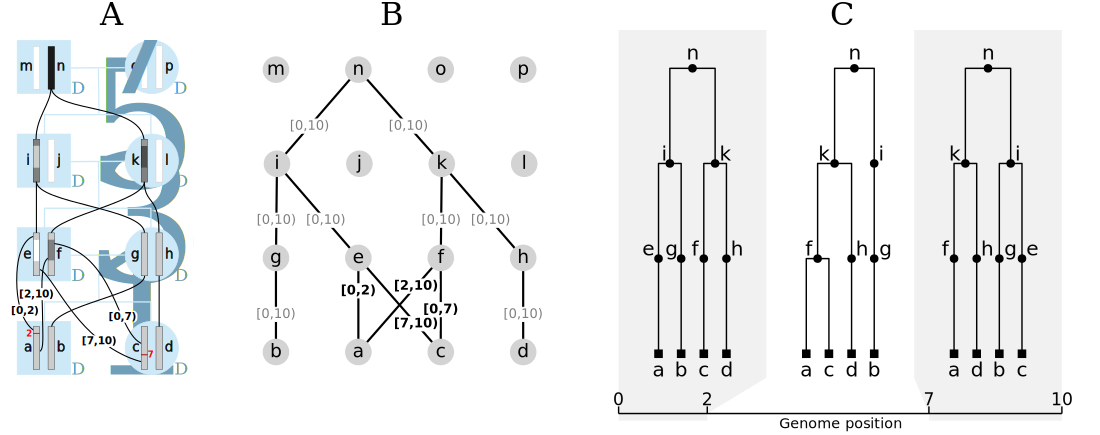
\includegraphics[width=\textwidth]{illustrations/arg-in-pedigree}
\end{center}
\caption{\label{fig-arg-in-pedigree}
% TODO caption needs another pass. Once the full section has been written
% it'll be clearer what we need to say in the caption vs the text.
An example genome ARG (gARG) embedded in a pedigree.
(A) Diploid individuals (blue), visualised in a highly inbred pedigree and
labelled $D_1$ to $D_8$,
contain both paternal and maternal  genomes
labelled \noderef{a} to \noderef{p}. Black lines show inheritance paths connecting
genomes in the current generation (\noderef{a} to \noderef{d}) with their ancestors.
Genomes \noderef{a} and \noderef{c} are the product of two independent
recombination events (red) between
the paternal genomes \noderef{e}
and \noderef{f}, and regions of genome inherited are shown with shaded colour.
Genomes are shaded such that where, backwards in time,
they merge into a common ancestor, the merged region is darker.
(B) The corresponding gARG along with inheritance annotations on all edges
(partial inheritance in bold).
(C) The corresponding local trees.
}
\end{figure}

As illustrated in Fig.~\ref{fig-arg-in-pedigree},
the gARG for a given set of individuals is embedded in their pedigree.
The pedigree relationship between the diploid individuals is
shown, along with their paths
of genetic inheritance and constituent genomes (labelled
with lowercase alphabetical letters
rather than integer identifiers to avoid confusion with genomic
intervals).
Thus, individual $D_1$ is composed
of genomes \noderef{a} and \noderef{b}, which are inherited from its
two parents, $D_3$ and $D_4$. Each inherited genome may be the recombined product
of the genomes
% FIXME "contained within" is a poor phrase here, use "constituent" or something
contained within a parent.
In this example,
genome \noderef{b} was inherited directly from $D_4$'s genome \noderef{g} without
recombination, whereas
genome \noderef{a} is the recombinant product of
$D_2$'s genomes \noderef{e} and \noderef{f} crossing over at position 2.
Specifically, genome \noderef{a} inherited the (half-closed)
interval $[0, 2)$ from genome \noderef{e} and $[2, 10)$ from genome \noderef{f}.
These intervals are shown attached to the corresponding graph edges.
The figure shows the annotated pedigree with realised inheritance of genomes
between generations, the corresponding gARG, and finally the corresponding
sequence of local trees along the genome.
The local trees represent the genealogy of genomes \noderef{a}--\noderef{d},
which changes between local trees due to recombination.
The local trees span the three genome regions delineated
by the two recombination breakpoints that gave rise to these genomes.
Following the above definitions, corresponding data encoding for
this gARG is shown in Tab.~\ref{tab-gARG-data} (Appendix~\ref{sec-gARG-data}).

These definitions follow naturally from the outcome of events
associated with the inheritance of DNA between generations.
% FIXME this sentance doesn't follow well from the first, needs a
% different bridge before listing important properties.
% Maybe the "listicle" format here isn't right anyway.
As such,
there are some important consequences to these definitions.
Firstly, there is
no limitation on a mating system, ploidy, or age structure in a gARG.
By making the
basic unit an individual's genomes,
any pattern of inheritance among mixed ploidy (e.g.\ haplodiploid
species) can be accommodated.
Secondly, because we record the intervals of inheritance
between genomes,
arbitrary patterns of genetic inheritance can be directly expressed, such as
gene conversions,
multiple simultaneous recombinations,
and so on.
% Wilder: give forward ref to section on efficiency here, mention tree sequence
% TODO, should probably drop this point.
Thirdly, local trees that we generate for a particular position on the
genome can have nodes of any arity (number of child nodes), including ``unary''
nodes with a single child (see Section~\ref{sec-locally-unary-edges}).
% TODO should rephrase this from parent/child to ancestor/descendant?
Fourth, recombination is modelled in terms of
its inputs (parental genomes) and output (child genome) with associated inheritance intervals.
Thus we will have a child node (the recombinant; e.g.\ node \noderef{a}
Fig.~\ref{fig-arg-in-pedigree}) and two (or more; see Section~\ref{sec-ARG-simplification})
% TODO: check above if we want to refer to sec-ARG-simplification or some other!
parental nodes from which this child has inherited genome segments.
% TODO rephrase the above, it'll confuse people. Just need to reiterate the
% points about events, and maybe lead into the next section
Finally, gARGs are not defined in terms of the
coalescent with recombination (or any other) stochastic process.
Thus, the gARG encoding is focused on faithfully representing the
\emph{outcome} of the processes of genetic inheritance
with recombination,
and is agnostic to the details of those processes.

% Firstly, a gARG may contain nodes that are both samples \emph{and}
% internal nodes in the local trees.
% This ability is useful when we have pedigree information
% along with genetic data
% \cite[e.g.][]{hayes20191000,RosFreixedes2022,anderson2022genes},
% where we may have many generations of internal sample nodes
% whose genomes have been sequenced.
% Another situation in which it is important that
% we do not assume samples are all contemporary ``leaf'' nodes
% (or that all internal nodes are either coalescences or recombinations)
% is when we are incorporating ancient genomes into ARG
% inference~\citep{speidel2021inferring,wohns2022unified}.
% Similarly, a gARG may contain nodes that
% do not correspond to any particular event in the ancestry of the samples.
% For example, node \noderef{h} is the direct ancestor of \noderef{d} in
% Fig~\ref{fig-arg-in-pedigree}, and is not the product of either a
% coalescence or a recombination. Such nodes would usually be removed
% from the graph so that \noderef{d} descends directly from \noderef{k} (see
% the ``\nameref{ARG_simplification}'' section) but there is no necessity for this from
% a representational perspective.
% Secondly, because we do not classify nodes by event type
% (common ancestor or recombination) there is no limitation
% on the complexity that can be modelled---multiple recombinations
% and coalescences can happen simultaneously in the same genome,
% a common occurance in large deeply sequenced
% pedigrees~\citep{hayes20191000,RosFreixedes2022}.
% Finally, there is a subtle and important point about how recombination
% is represented: which genome in the organismal lifecycle
% do nodes represent?
% In principle, we can interpret nodes as representing genomes
% at any point in the life cycle [supplementary Figure ?]. Hudson
% views nodes as representing gametes~\citep{hudson1983properties}.
% However, we argue that the most intuitive
% approach is to let nodes represent the genomes present in diploid
% individuals in each generation, as in
% Fig~\ref{fig-arg-in-pedigree}A. In this case recombination
% is not represented by a single ``recombination node'' (as in an eARG), but with
% two parent genomes between which recombination takes place
% (e.g.\ nodes \noderef{e} and \noderef{f}), and a
% single resulting ``recombinant'' genome (e.g.\ \noderef{c}). The
% edges that link this recombinant with its two parents carry the information
% concerning breakpoint location that would be associated with a
% recombination node in an eARG. [TODO finish up here with more
% clarity on what this means in terms of the required specifity
% of recombination events, and put in a forward ref to the simplification
% section where we talk about stacking up recombination events
% and their identifiability.]


\section{Event ARGs}
\label{sec-eARG}
% FIXME - this intro doesn't work at all now - we haven't defined what an
% eARG *is* before discussing it.
% Maybe best to skip this entirely, and make the quoted definitions with
% a thin intro the way to start the section.
Genome ARGs are defined by
describing the details of genetic inheritance
between ancestor and descendant genomes.
In contrast, ARGs are classically defined
by describing the \emph{events} in the history of a sample of genomes.
The difference between gARGs and the prevalent views of eARGs
% what defines an ARG
are subtle and difficult to distinguish.
It is therefore useful to first survey some representative
recent definitions of
an ARG from the literature, to allow us to capture their common features
(see Appendix~\ref{sec-arg-history} for a full review).

\citet{brandt2021evaluation} follow the original Griffiths definition of
an ARG by coupling it directly to a generative process, stating
that the ``full ancestral recombination graph (ARG) is a structure that encodes all
coalescence and recombination events resulting from the stochastic process of
the coalescent with recombination.''
\citet{shipilina2023origin} emphasise the true existence of the
corresponding events (rather than the generative process) by saying that
``[t]he ARG describes the complete
ancestry of a sample of genomes through a series of real coalescence and
recombination events.''
\cite{mathieson2020ancestry}
define an ARG as ``a subset of the pedigree...
contain[ing] only those edges along which inherited segments of DNA have been
transmitted, and only those nodes corresponding to ancestors in which there was
a recombination or coalescence event.''
% In contrast, ~\citet{gusfield2014recombinatorics} defines an ARG as [TODO]
% Papers that do not discuss how positions work:
% - Mathieson and Scally: no discussion of how it works concretely (but quite
%   close to gARG, in some ways)
% TODO list out some of these as examples of where people don't bother
% getting into this important detail?

% NOTE: important to emphasise TWO things here, events and vagueness
% actual encoding mechanism (i.e. how trees fit into the ARG)
A common feature of these definitions is that they are expressed
in terms of evolutionary \emph{events}, and so for the purposes of
discussion we can label
this prevailing interpretation as an ``event ARG'', or eARG.
(Many definitions also emphasise
the necessity of exhaustively capturing \emph{all} events, which we
examine in later sections.)
Another common feature of these definitions is that they do not explicitly
discuss the mechanism by which local trees vary along the genome.
The topology of an eARG defines the common ancestor and
recombination events that occurred,
but the graph structure alone is not sufficient to define the local trees,
or equivalently, how ``ancestral material'' flows along
the edges of the ARG (see Section~\ref{sec-eARG-to-gARG}).
% TODO: check above if we want to refer to sec-eARG-to-gARG or some other!
This is usually assumed to follow the mechanism described by
Griffiths and colleagues in which we have
two different ``types'' of node in the graph:
common ancestor nodes in which the inbound lineages are merged into a
single ancestral lineage with one parent, and recombination
nodes in which a single lineage is split into two independent
ancestral lineages.
Recombination nodes are then
annotated with
the corresponding crossover breakpoint~\citep{griffiths1996ancestral}.
Fig.~\ref{fig-event-arg} shows an example of a classical
eARG with three sample genomes (\noderef{a}, \noderef{b}, and \noderef{c})
and a single recombination event,
% Trying to emphasise here that this is just an example data encoding.
% I can imagine
% people nitpicking about how this specific way of doing it is bad
% for reason X.
along with an example encoding of the data.
There is a single recombination event
at node \noderef{d} with a breakpoint at position $x$. We
assume that \noderef{d} inherits genetic material to the
left of $x$ from \noderef{e} and to the right of $x$ from \noderef{f}.
As shown in Fig.~\ref{fig-event-arg}B,
the local trees are embedded in the graph, and can be reconstructed
in essentially the same manner as outlined in the previous section for
gARGs. The only difference is that decisions about which outbound
edge to follow during the rootward traversal are taken at recombination
nodes, following
either the common convention that the order of parents
is significant~\citep[e.g.][]{griffiths1991two},
or by incorporating additional information to
distinguish left and right parents
into the
encoding~\citep[e.g.][]{gusfield2014recombinatorics,ignatieva2021kwarg}.
% JK: not sure what you're getting at here Gregor? The ordering matters
% because you have to write each event down precisely.
% Gregor: Importantly, the order of events matters to WHAT!?

\begin{figure}
\centering
\tikzmath{\x1 =0; \x2=8;\xx=12.5; \x3=14; \xt=18;}
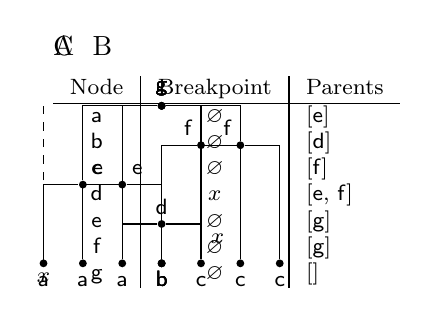
\begin{tikzpicture}[x=5mm, y=5mm, node distance=2mm and 20mm]
\tikzset{greynode/.style={circle,fill,inner sep=1},
nodelabel/.style={font=\footnotesize}}


\node [anchor=north west] at (\x1,6) {A};
\node [anchor=north west] at (\x2,6) {B};
\node [anchor=north west] at (\xt,6) {C};

%%% (A) ARG

\node (s0) [greynode] at (\x1 + 0, 0) {};
\node (s1) [greynode] at (\x1 + 3, 0) {};
\node (s2) [greynode] at (\x1 + 6, 0) {};
\node (s3) [greynode] at (\x1 + 3, 1) {};
\node (s4) [greynode] at (\x1 + 1, 2) {};
\node (s5) [greynode] at (\x1 + 5, 3) {};
\node (s6) [greynode] at (\x1 + 3, 4) {};

\draw (s1) -- (s3);
\draw (s0) |- (s4);
\draw (s4) -- (\x1 + 2,2) |- (s3);
\draw (s4) |- (s6);
\draw (s3) -- (\x1 + 4,1) |- (s5);
\draw (s2) |- (s5);
\draw (s5) |- (s6);

%%% (B) Trees
\node (l0) [greynode] at (\x2 + 0, 0) {};
\node (l1) [greynode] at (\x2 + 2, 0) {};
\node (l2) [greynode] at (\x2 + 3, 0) {};
\node (l3) [greynode] at (\x2 + 1, 2) {};
\node (l4) [greynode] at (\x2 + 2, 4) {};

\draw (l0) |- (l3);
\draw (l1) |- (l3);
\draw (l2) |- (l4);
\draw (l3) |- (l4);

\node (r0) [greynode] at (\x3 + 0, 0) {};
\node (r1) [greynode] at (\x3 + 1, 0) {};
\node (r2) [greynode] at (\x3 + 3, 0) {};
\node (r3) [greynode] at (\x3 + 2, 3) {};
\node (r4) [greynode] at (\x3 + 1, 4) {};

\draw (r0) |- (r4);
\draw (r1) |- (r3);
\draw (r2) |- (r3);
\draw (r3) |- (r4);

\foreach \u/\lab in {
        s0/$\noderef{a}$, s1/$\noderef{b}$, s2/$\noderef{c}$,
        r0/$\noderef{a}$, r1/$\noderef{b}$, r2/$\noderef{c}$,
        l0/$\noderef{a}$, l1/$\noderef{b}$, l2/$\noderef{c}$}
    \node[nodelabel,anchor=south] at ([yshift=-12pt]\u) {\lab};

\foreach \u/\lab in {
        s6/$\noderef{g}$,
        l4/$\noderef{g}$,
        r4/$\noderef{g}$}
    \node[nodelabel,anchor=south] at (\u) {\lab};

\node [nodelabel,anchor=north west] at ($(s3) + (\x1 + 0,0)$) {$x$};
\foreach \u/\lab in {
        s4/$\noderef{e}$,
        l3/$\noderef{e}$}
    \node[nodelabel,anchor=south west] at (\u) {\lab};
\foreach \u/\lab in {
        s5/$\noderef{f}$,
        r3/$\noderef{f}$}
    \node[nodelabel,anchor=south east] at (\u) {\lab};
\foreach \u/\lab in {s3/$\noderef{d}$, s6/$\noderef{g}$}
    \node[nodelabel,anchor=south] at (\u) {\lab};

\draw[dashed] (\xx,0) -- (\xx, 4);
\node[nodelabel,anchor=north] at (\xx,0) {$x$};


%%% (C) Encoding
\node [nodelabel,anchor=north west] at ($(\xt,5)$) {
\begin{tabular}{c|c|l}
% \multicolumn{2}{c}{Breakpoints}\\
Node & Breakpoint & Parents\\
\hline
$\noderef{a}$ & $\varnothing$ & [\noderef{e}]\\
$\noderef{b}$ & $\varnothing$ & [\noderef{d}] \\
$\noderef{c}$ & $\varnothing$ & [\noderef{f}]\\
$\noderef{d}$ & $x$ & [\noderef{e}, \noderef{f}] \\
$\noderef{e}$ & $\varnothing$ & [\noderef{g}]\\
$\noderef{f}$ & $\varnothing$ & [\noderef{g}]\\
$\noderef{g}$ & $\varnothing$ & []\\
\end{tabular}};

\end{tikzpicture}
\caption{\label{fig-event-arg}
A classical event ARG. (A) Standard graph depiction with
breakpoint $x$ associated with the recombination node \noderef{d}.
Nodes \noderef{e}, \noderef{f} and \noderef{g} are common ancestor events.
(B) Corresponding local trees to the left and right of breakpoint $x$
(note these are shown in the conventional form in which only coalescences
within the local tree are included; see Section~\ref{sec-ARG-and-local-trees}
% TODO: check above if we want to refer to sec-ARG-and-local-trees or some other!
for a discussion of this important point).
(C) A concrete encoding of the information.
Recombination nodes have a non-null breakpoint
and two parents.
}
\end{figure}

% TODO reference forward to the cell ARG appendix. Ultimately
% every event corresponds to a particular genome in a particular
% individual or cell.
Whether we regard nodes as events or genomes is something of a
philosophical question, and in most senses the two are equivalent
(but see the discussion on ``unary nodes'' in Section~\ref{sec-locally-unary-edges}).
From a concrete data-structure encoding perspective, the only real
difference between an eARG and a gARG is that in an eARG we store recombination
\emph{breakpoints} at nodes of out-degree two (recombination nodes)
whereas in a gARG we store \emph{inheritance intervals} on edges.
A key advantage of associating inheritance intervals with
edges in a gARG is that it allows us to describe genetic inheritance events other
than simple crossovers, such as multiple recombinations and
gene conversions. By explicitly stating the exact regions of genome
that are transmitted along an edge, we generalise the representation
to encompass any process that leads to the differential inheritance of
genetic material along the genome.

While the additional generality provided by the gARG representation
is useful, it is in reality a small change that does not
lead to significantly different time or space complexity in computational
tasks.
The vitally important and fundamental distinction between
a gARG and an eARG is that gARGs
allow us to directly describe
genetic inheritance in multiple non-contiguous genome intervals
between an ancestor and a descendant, which cannot be done
by specifying recombination events and breakpoints.
% FIXME this sentence is problematic. We should recast to talk about
% the outcomes of events, not talk about simulateousness (which will
% confuse people
Thus, we have the means to encode the \emph{outcome} of
multiple genetic inheritance events, and to
systematically describe the uncertainty around their
ordering (see Section~\ref{sec-precision}).
As we describe in the following sections, freeing ourselves from the requirement
of recording specific events and
the additional generality of the gARG encoding
has significant advantages. It also raises questions about what our goals
for inferring ARGs should be, and how we evaluate the success
of such inferences.

\section{Retrospective vs prospective ARGs}
\label{sec-retro-pro}
The ARG concept arose from a \emph{retrospective} view of inheritance.
For example the definition of an eARG, as discussed above, is invariably
couched in terms of the events that occured in the history of some set of sampled
genomes. Similarly, the genome ARG in Fig.~\ref{fig-arg-in-pedigree}
is retrospective because it only includes information
about genetic inheritance relative to the sample individuals
$D_1$ and $D_2$ (genomes \noderef{a}--\noderef{d}).
That is, only the inheritance
history of the sample genomes \noderef{a}--\noderef{d} is recorded in the ARG.
% Gregor & Jerome think that "inheritance" is clearer here than "transmission"
Genetic inheritance must have occurred between (e.g.)
$D_8$ and her daughter $D_6$, but this is not recorded because
it is not relevant to the genetic ancestry of the sample genomes.

There is no particular reason, however, that ARGs must be
retrospective. Recent advances in individual-based forward-time simulation
~\citep{kelleher2018efficient,haller2018tree} depend upon the ability to
record gARGs in a \emph{prospective} manner.
In a prospective gARG, the inheritance intervals $I$
on an edge joining ancestor genome $v$ and descendant $u$
define \emph{all} regions of genome that $u$ inherited from $v$.
Thus, these inheritance intervals are
concerned only with the genetic relationship
between the nodes in question, and are not defined with respect
to any given set of samples. They simply record the immediate
genetic inheritance between two genomes
(in the simplest case, between a parent and a child).
\citet{kelleher2018efficient} refer to the structure
recording all such forwards-in-time genetic relationships
as an ``embellished pedigree`` (and suggest the term ``nedigree'' as a shorthand).
Describing this instead as a ``prospective ARG'', emphasising
the use of the same data structures and the direct connection with
the usual retrospective interpretation of an ARG, may be
more useful.

The exhastive recording of full inheritance intervals from generation
to generation leads to a rapid build-up of information, much of which
may not be relevant to the genetic ancestry of the current population.
This redundancy can be periodically removed using the ``simplify'' algorithm,
described in detail by \citet{kelleher2018efficient}. Simplification
allows efficient subsetting of ARGs (removing both samples and certain
levels of detail about recombination, as discussed in Section~\ref{sec-ARG-simplification}),
and is also the key enabling factor when incorporating propective ARGs into
forward-time simulation.
The core algorithm involves the concept of
``ancestral material''~\citep{wiuf1999ancestry,wiuf1999recombination}:
the genomic intervals ancestral to a set of samples,
scattered across lineages (the edges of the graph)
at some time in the past. In the next section, we outline how
tracing ancestral material allows the identification and removal of nodes
and inheritance intervals, such that
only genetic ancestry relevant to the current population is retained.

\section{Converting an eARG to a gARG}
\label{sec-eARG-to-gARG}
Any eARG can be converted to a gARG without loss of information.
The process is illustrated in Fig.~\ref{fig-ancestry-resolution} (A to B):
we convert all event nodes to genome nodes and add inheritance annotations
to the gARG's edges. If the node is a common ancestor node,
we annotate the single outbound edge with the interval $[0,L)$,
for a genome of length $L$.
If the node is a recombination event with a breakpoint $x$,
we annotate the two outbound edges respectively with the intervals $[0, x)$ and $[x, L)$.
These inheritance interval annotations are clearly in one-to-one
correspondence with the information in the input eARG.

\begin{figure}
\centering
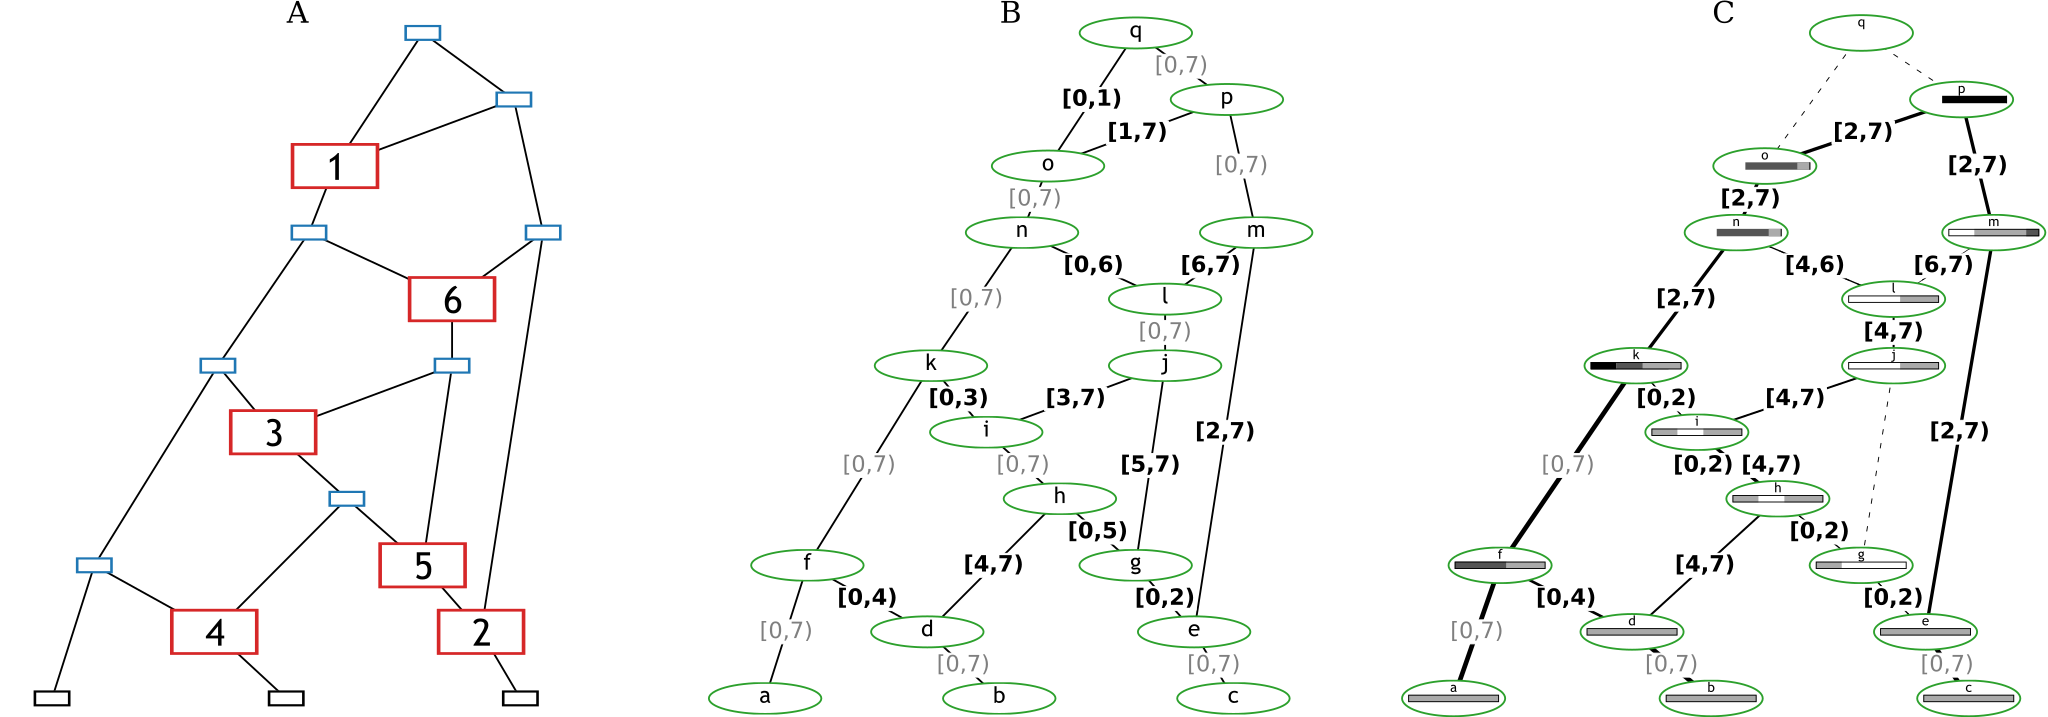
\includegraphics[width=\textwidth]{illustrations/ancestry-resolution}
\caption{\label{fig-ancestry-resolution}
Converting the \citet[][Fig.~1]{wiuf1999recombination} example
to a sample-resolved gARG. (A) The original eARG; square nodes represent events, with
each recombination (red) containing a breakpoint.
(B) The corresponding gARG with breakpoints directly converted to
edges annotated with inheritance intervals.
(C) The sample-resolved gARG resulting from simplifying with respect
to the sample genomes, \noderef{a}, \noderef{b}, and \noderef{c}.
Dashed lines show edges that are
no longer present (in practice, nodes \noderef{g}, \noderef{j}, and \noderef{q} would also be removed).
Coalescence with respect to the sample is indicated by shaded bars, as
in Fig~\ref{fig-arg-in-pedigree}A; nodes \noderef{n}, \noderef{o}, \noderef{p}, \noderef{q} have incomplete
bars showing that local ancestry of entirely coalesced regions is omitted.
Line thickness is proportional to the genomic span of each edge.
Nodes representing recombination events are retained
for clarity, but could be removed by simplification if
desired.
}
\end{figure}

This way of specifying inheritance intervals generates annotations equivalent to
those produced in a prospective gARG, and which is similarly amenable to ``simplification'',
by considering the genetic material that is ancestral to the samples \citep{kelleher2018efficient}.
The outcome of this process, which is
directly analogous to Hudson's simulation algorithm for the coalescent with
recombination~\citep{hudson1983testing,kelleher2016efficient}, is shown in
Fig.~\ref{fig-ancestry-resolution}C. We traverse from the samples rootwards through the graph
keeping track of which material is ancestral to the samples.
At recombination events, ancestral material is split between the ancestral lineages.
As genome segments coalesce in a common
ancestor the total amount of ancestral material is reduced, until
eventually all samples reach a most recent common ancestor at every location
along the genome.

Fig.~\ref{fig-ancestry-resolution}C therefore represents a \emph{sample-resolved} gARG,
% useful to say that we don't *need* to simulate an eARG and convert to a
% sample-resolved form, but can simulate a sample-resolved gARG directly
of the sort that can be simulated directly by the Hudson algorithm.
This differs in some important ways from its equivalent eARG (Fig.~\ref{fig-ancestry-resolution}A).
Firstly, we can see that some nodes and edges have been removed entirely
from the graph.
The ``grand MRCA'' \noderef{q} is omitted from the
sample-resolved gARG because all segments of the genome have
fully coalesced before it is reached. Likewise, the edge
between \noderef{g} and \noderef{j} is omitted because the recombination
event at position $5$ (represented by node \noderef{g})
fell in non-ancestral material.
More generally, we can see that the sample resolved
gARG of Fig.~\ref{fig-ancestry-resolution}C
allows for ``local'' inspection
of an ARG in a way that is not possible by storing
common ancestor and recombination events in an eARG. Because
the ancestral material is stored with each edge, the
cumulative effects of events over time can be reasoned
about, without first ``replaying'' those events. Many computations
that we wish to perform on an ARG will require resolving
the ancestral material with respect to a sample.
% this is weak, but would be good to emphasise this point.
% you just end up running simplify lots of times, in your
% downstream algs
The gARG encoding
allows us to perform this resolution of ancestral material once
and to store the result,
whereas the eARG encoding requires us to repeat the process
each time.

Note that the \citet{wiuf1999recombination} eARG
in Fig.~\ref{fig-ancestry-resolution} is not particularly
representative, because inference or simulation methods will usually
only generate ARGs containing nodes and edges ancestral to the sample
(see the discussion of the ``Big ARG'' stochastic process in
Appendix~\ref{sec-big-and-little-arg}, however).
Nonetheless, it is an instructive example from the literature which highlights several
important properties of ARGs, and the general point about
the need to resolve ancestral material ``on the fly'' for eARG traversals
holds.

\section{ARGs and local trees}
\label{sec-ARG-and-local-trees}
Local trees, describing the genetic genealogy of a sample
at a particular location along the genome, are
embedded within an ARG, and the relationship
between the two is subtle and important.
Note that many authors use the term ``marginal''
% could list loads here, but not much point.
trees~\citep[e.g.][]{griffiths1996ancestral,minichiello2006mapping,kelleher2016efficient}
which we avoid due to the potential confusion with the
statistical concept of marginal distributions
(potentially leading to interpretation as an integrated tree over many positions).

% TODO Need to make clear here what came from where. Basic combinatorial object
% cite Knuth. Application to genetic ancestry, sim papers. Need to look
% up what's said in favour of this integer based approach in which paper
% and refer to tat.
To make the following discussions precise, we provide
a concrete definition and explicit process for local tree extraction.
We can describe a local tree as an
oriented tree~\cite[p.\ 461]{knuth11combinatorial},
a sequence of integers $\pi_1, \pi_2\dots$ where $\pi_u$ denotes the parent of
node $u$~\citep{kelleher2013coalescent,kelleher2014coalescent,kelleher2016efficient}.
If $u$ is a root
% I'm not sure if this reachability stuff is a helpful clarification, and whether it'll just
% confuse people. It depends on some tricky details.
(or not reachable from the samples)
in the local tree at position $x$, then we adopt the convention that $\pi_u = -1$.
% TODO Give example of an oriented tree from one of the figs?
% TODO
% A node in an oriented tree can have
% zero, one,
% or many children.

To recover the local tree $\pi$ at position $x$, we begin by
setting $\pi_u = -1$ for each $u\in N$. Then, for each sample
node in $S$ we trace its path rootwards through the
ARG for position $x$, and record this path in $\pi$.
Specifically, at a given node $u$,
we find an edge $(c, p, I) \in E$ such that $u = c$ and $x \in I$, and set
$\pi_c \leftarrow p$. We then set $u \leftarrow p$, and repeat
until either $\pi_u \neq -1$ (indicating we have traversed this section
of the ARG already on the path from another sample) or there
is no matching outbound edge (indicating we are at a root).

The nodes in a local tree encoded
in this way are \emph{labelled} (i.e.\ carry the identity
of the corresponding ARG node), and this is fundamentally
important to how a local tree relates to its ARG.
If we are given the sequence of local trees for a gARG
encoded as an oriented tree (or in any other form in which
the tree nodes are explicitly labelled with the identity of the
corresponding ARG node),
along with the genome interval covered by each tree,
then we can recover precisely the same ARG. Thus, under this
definition, there
is a one-to-one correspondence between an ARG and
the sequence of local trees that it encodes.

This is not the prevailing view, however.
\cite{kuhner2017consensus} argue that the
``interval-tree'' representation of
an ARG (the local trees and the genome intervals they cover)
``does not contain all of the information in the underlying ARG: it lacks the
number of recombinations occuring at each site, the times at which
recombinations occurred, and the specific sequences involved as recombination
partners.''
\cite{shipilina2023origin} discuss the same ideas,
and note that the
``full ARG...~contains more information than the series of tree
sequences along the genome''.
These statements that an ARG
contains more information than its local trees is only true
if we use a representation of the local trees that discards
information about those local trees that can be derived from the ARG.
The internal nodes of evolutionary trees are usually
considered to be \emph{unlabelled}
because they most often correspond
to anonymous hypothetical ancestors.
Internal ARG nodes may likewise correspond to anonymous hypothetical
ancestors, but if we do not label the tree nodes we lose the fact that
the \emph{same} ancestors persist across multiple trees.
Besides having labelled nodes, the local trees must contain
unary nodes marking recombinations
and other processes that lead to lineages passing through a given
ARG node without coalescence in the local trees
(see Section~\ref{sec-locally-unary-edges}).
If the local trees contain labelled internal nodes, they precisely
describing the corresponding path through the graph for each
genome interval and there is exactly as
much information in them as in an ARG.

These properties have interesting consequences when we
consider the inference strategy of estimating local trees
% TODO rephrase this. Ana doesn't like the way it implies that the
% trees are independent, because info from mutations outside the
% window are shared. However, each tree *inference* is independent,
% whether information is used multiple times in different trees or not
independently within genome segments,
and subsequently stitching them together into an ARG.
Two recent methods take this approach,
\relate~\citep{speidel2019method} and
\espalier~\citep{rasmussen2022espalier},
and have different strategies for reconciling the local trees into an ARG.
\relate\ first infers local tree topologies, and then identifies
edges that persist from tree to tree by reasoning about the sets of samples
subtended. It does not attempt to be exhaustive.
\espalier, on the other hand, is specifically interested
in the details of recombination events (among a small number of samples)
and therefore attempts to infer
the precise subtree prune-and-regraft (SPR)
operations~\citep{hein1990reconstructing,song2003on,song2006properties}
induced by recombination.
Inferring the SPRs between leaf-labelled trees is
NP-hard~\citep{hein1996complexity,allen2001subtree,bordewich2005computational},
but it is unclear what the complexity is when there
is a degree of internal node sharing between trees.

\section{Locally unary nodes}
\label{sec-locally-unary-edges}
We can define the arity of a node as the number of child nodes it has.
There is an
important distinction between the number of children a node has
in the graph and the number of children it has in the local trees,
because a (graph) child node is only a child in the local tree for position
$x$ if $x$ is in the inheritance interval for the corresponding edge.
Thus, for a given node $u$ and a genome position $x$ the arity
of $u$ in that local tree is less than or equal to the graph arity of
$u$. The arity
of a node in the local trees can therefore change as we move along
the genome.

This distinction between graph and local tree arity is mainly
of interest when we consider \emph{unary} nodes, those that have
a single child.
Returning to the example in Fig~\ref{fig-arg-in-pedigree}, nodes
\noderef{g} and \noderef{h} are ARG-unary (Fig~\ref{fig-arg-in-pedigree}B), and are consequently
also unary in the local trees (Fig~\ref{fig-arg-in-pedigree}C).
On the other hand, node \noderef{f} has two children
in the graph, but is binary only
in the local tree covering the interval $[2, 7)$,
representing the coalescence of samples \noderef{a} and \noderef{c}
in this region of genome. Over the interval $[0, 2)$ no coalescence occurs,
but we still record the fact that genome \noderef{c} inherits from \noderef{f}
in the local tree. Thus, \noderef{c} has a single child in this
interval and it is hence unary in this local tree.
In another example, \noderef{e} is binary in the graph, but is
unary in each of the local trees in which it is present.
This is because \noderef{a} and \noderef{c} are both recombinant
offspring of \noderef{e} and \noderef{f}, and,
in this example,
\noderef{a} inherits from
\noderef{e} over the interval $[0, 2)$,
and \noderef{c} inherits from \noderef{e} over $[7, 10)$.
The intervals over which
we know that a node inherits from another, but where there
is no local coalescence, are marked by unary nodes in the
local trees.

Outside of the context of simulation, ARG-unary nodes are
only like to occur in longitudinal datasets where genetic
data is sampled at many timepoints and recombination
is rare (e.g.~SARS-Cov-2; see Discussion).
\emph{Locally} unary nodes, those which have one child
in one or more local trees, are a common and important feature
of many different types of ARG, and a recurring topic
in this article. Without these nodes marking the passage
of ancestral material through specific ancestors, the local trees
lack information about events other than local coalescence.
% Not sure if switching example will confuse people here, but would
% like to contrast with example where we don't use unary nodes to
% emphasise the point that we lose info
For example, the local trees for the classical event ARG
depicted in Fig.~\ref{fig-event-arg}B follow the usual conventions
and do not include any information about the recombination
that occurred at node \noderef{d}. Given these two local trees
in isolation
% (without further information about the corresponding ARG)
we lack specific information about the recombination.
Explicitly recording that node \noderef{d} lies on the
branch joining \noderef{b} to \noderef{e} in the left hand
tree, and \noderef{b} to \noderef{f} in the right hand tree
resolves all ambiguity, and makes the collection of local
trees exactly equivalent to the corresponding ARG (see previous section).
Unary nodes are a vital link between ARGs and local trees, and we
cannot fully reason about how a local tree is embedded in an ARG
without them.

Nodes with one child are not a standard feature of evolutionary trees
or the ARG literature
(although \citet{mathieson2020ancestry} show examples in which the ARGs
contain unary nodes, and state that paths are
``implicitly passing through points representing specific individuals.'').
We are usually interested in
nodes that have at least two children because these
are in principle detectable from mutational differences
arising in the respective subtrees.
A tree branch may correspond to many generations
of individuals (or indeed cell divisions; see Appendix \ref{sec-cell-lineages-and-args})
and there is usually
little information about these intermediates, and hence limited utility
in modelling them.
As we see in the next section, however, there is a range of
different ways in which ARG nodes can be locally unary. Furthermore,
several current ARG inference methods infer locally unary nodes
(see Section~\ref{sec-precision}).

\section{Levels of simplification}
\label{sec-ARG-simplification}
ARG simplification is a powerful tool, and can do far more
than removing unreachable nodes and edges in a prospective ARG
and resolving ancestral material in an eARG.
In general, we can think of
ARG simplification as the process
of removing nodes and re-writing edges (and their inheritance annotations)
to remove various types of redundancy.
The redundancy that we are interested in
% We are interested in both graph and local unary, so qualifying this
% would just make it less readable, IMO
revolves around the presence of unary nodes (see previous section).
We illustrate this successive removal of redundancy
through a series simplification steps
in Fig.~\ref{fig-simplification}.

\begin{figure}
\centering
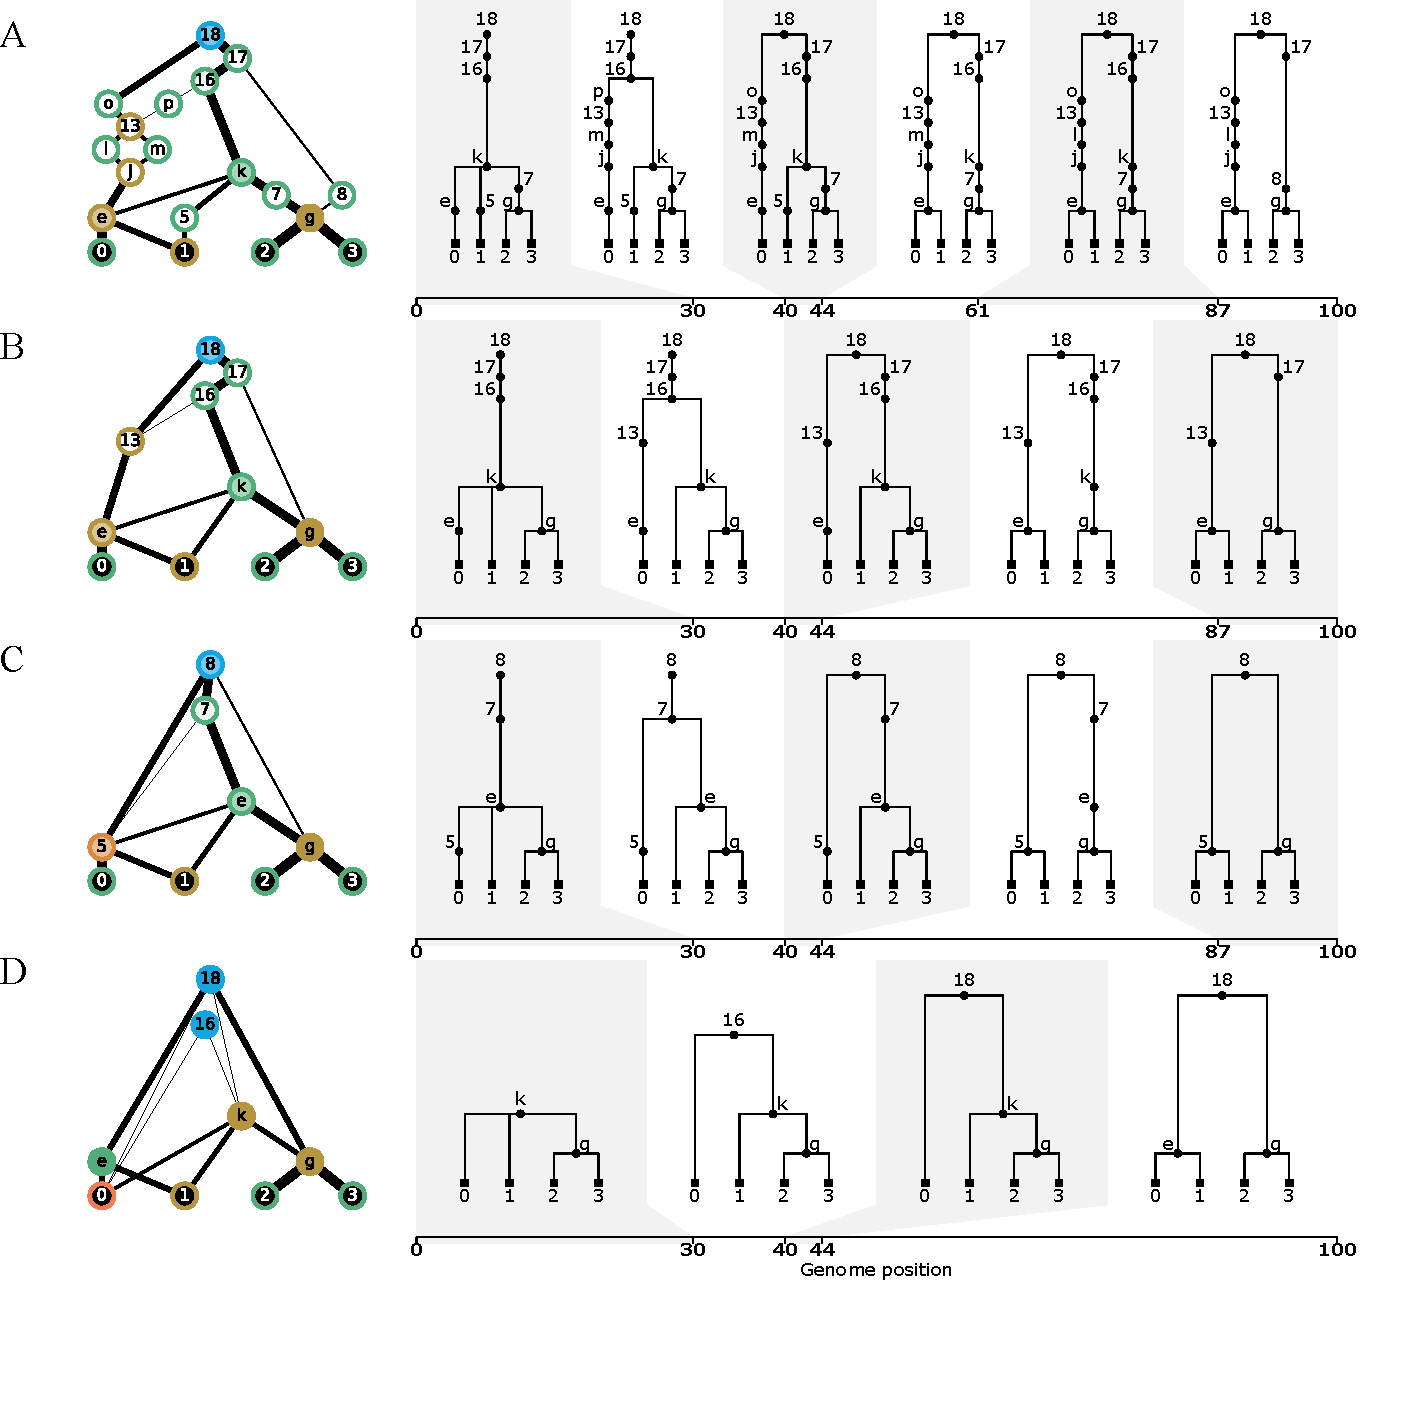
\includegraphics[width=\textwidth]{illustrations/simplification}
\caption{\label{fig-simplification}
Levels of ARG simplification.
(A) An example ARG simulated from a diploid Wright-Fisher model.
(B) Remove all
singly-connected graph components (e.g., diamonds such as \noderef{jlnm}).
(C) Remove nodes that never represent coalescences,
i.e.\ are unary everywhere (e.g.\ \noderef{n} and \noderef{r}).
(D) Rewrite edges to bypass nodes in local trees in which they are unary.
In each case, the graph is shown on the left
and corresponding local trees on the right.
Graph nodes are coloured by the number of parents and shaded
according to the proportion of their span over which they are coalescent;
see the text for more details.
}
\end{figure}

The ARG in Fig.~\ref{fig-simplification}A is the output of a
backwards-time Wright-Fisher simulation for a sample of two diploid
individuals (population size $N=10$), and follows a similar process
to the methods described by~\cite{nelson2020accounting}.
As we proceed backwards in time, generation by generation, the
extant lineages chose parents randomly.
With a certain probability recombination occurs, and the ancestral
material of a lineage is split between the two parental
genomes. Local coalesence occurs
when lineages with overlapping ancestral material choose the same
parent genome.
Note that in this simulation we do not explicitly
model recombination \emph{events} via an ARG node, but simply record
the \emph{outcome} of a recombination via outbound edges to
the parent's two genomes.
Thus, a recombinant node may also correspond to a coalescence
(e.g.~node \noderef{g} in Fig.~\ref{fig-simplification}).
The distinction of
using a single node to represent
a recombination event (e.g.~Fig~\ref{fig-ancestry-resolution}),
or two to represent the parent genomes is usually not important
(either is possible in the gARG encoding)
and the most convenient approach will vary by application.
Note also that polytomies are a natural feature of such
a Wright-Fisher model
(e.g.~node \noderef{k} in Fig.~\ref{fig-simplification}).

Fig.~\ref{fig-simplification} shows four ARGs (A--D), with
the graph depicted on the left and the corresponding sequence
of local trees on the right. The graph visualisations have
some novel features, which require some explanation.
Firstly, edge weights (the thickness of the lines joining
nodes) correspond to the length of the inheritance intervals
they are annotated with. This allows us to distinguish
edges that persist across many local trees from those that are
less influential (contrast the edge
$(\noderef{g}, \noderef{h})$
with $(\noderef{g}, \noderef{i})$
in Fig.~\ref{fig-simplification}A).
% FIXME this needs some work
Secondly, node colours denote the number of parents that they
have in the graph, allowing us to easily see roots (those
with zero parents), recombinanants (those with two parents)
and more complex situations arising from simplification (see below).
Thirdly, the shading intensity of a node denotes the
fraction of the node's span (the length of genome in which it
is reachable from the samples in the local trees)
over which it is coalescent (has more than one child).
% This is useful why? I can't come up with a quick way of saying
% this. In some senses it's a measure of identifiability?
% JK: Hmm, not sure we want to jump into inferability here?
All these features will impact what kind of an ARG we can
hope to infer from sampled genomes.

Returning to the main topic of this section,
Fig.~\ref{fig-simplification}A is the direct output of a Wright-Fisher
simulation in which we retain all nodes involved in recombination
or common ancestry events. This is the true history, and contains
a very high level of detail, some of which may be considered
redundant (or, from another perspective, unobservable).
In Fig.~\ref{fig-simplification}A the local trees (right)
contain many unary nodes, and as we successively simplify,
the local trees contain fewer
unary nodes (Fig.~\ref{fig-simplification}B,C) until
we reach Fig.~\ref{fig-simplification}D, where the local trees
have no unary nodes.
A node is unary in a local tree covering the genome interval $I$
if genetic inheritance passes through that ARG node,
but no coalescence occurs in the interval $I$.
The distinction between the ``common ancestry'' of two or more genomes
in an ancestral genome and the ``coalescence'' which may or may
not occur in the local trees is
important~\citep{hudson1983testing,kelleher2016efficient}.
Consider \noderef{e} in Fig.~\ref{fig-simplification}A,
for example. We can see from the graph that it is a common
ancestor of samples \noderef{a} and \noderef{b}, but
it does not correspond to any coalescence in the
local trees to the left of position $44$, and is therefore
unary in these three trees.

The first level of simplification that we can perform is to remove
parts of the graph topology that are invisible to the samples.
An example of such topology is a
``diamond''~\citep{rasmussen2014genome}
in which the two parent nodes of a recombination immediately
join again into a common ancestor (e.g.~\noderef{j}, \noderef{l}, \noderef{m}
and \noderef{n} in Fig.~\ref{fig-simplification}A).
Unless we are specifically
interested in the recombination event or these ancestral genomes,
there is no information in this topology and the diamond can be
replaced by a single edge. More generally, any
subgraph that is singly-connected in both the leafward and
rootward direction (a ``super-diamond'') is non-identifiable and can be
replaced by one edge. This definition includes the case
of a node that has one inbound and one outbound edge, such as
nodes \noderef{f} and \noderef{h}.
Fig.~\ref{fig-simplification}B shows the result of this type of
graph topology simplification.

Simplifying away diamonds will remove many unary nodes from the
local trees, but there can still be nodes that are unary in all
of the local trees. In particular, a node can represent a recombinant
with multiple parents in the graph but only a single child (e.g.\ node \noderef{n}
in Fig.~\ref{fig-simplification}B), or can represent a common ancestor with
multiple children in the graph but in which no coalescence takes place
in the local trees
(node \noderef{r} in Fig.~\ref{fig-simplification}B).
% point out that this is why Hudson refers to CA nodes, not coalescence nodes
Such nodes are not singly connected in the graph, but are nevertheless unary in
all of the local trees.
The operation to remove them
therefore requires knowledge not just of the graph topology but also of the
ancestral material associated with the edges.
As we see in Fig.~\ref{fig-simplification}C,
removal of recombinant nodes can produce graph nodes with
more than two parents (e.g.~node \noderef{e}); and likewise, removal of
common ancestor but non-coalescent nodes can produce graph nodes with
more than two children (e.g.~node \noderef{s}). These represent the
merged
\emph{effects} of multiple evolutionary events in a single node (genome), and the
ARG no longer contains the intermediate genomes representing those events.

The remaining nodes are MRCAs of some subset of the samples
at \emph{some} positions along the genome. We still have
some unary nodes in the local trees, but these nodes will
correspond to a coalescence in at least one other
local tree. For example, node  \noderef{k} is unary in the fourth tree
of Fig.~\ref{fig-simplification}C, but is either binary
or ternary in all other local trees (recall this is a Wright-Fisher
simulation). The final level of simplification is to alter the edge annotations
such that, although no nodes are removed from the graph, all
unary nodes disappear from the local trees (Fig.~\ref{fig-simplification}D).
Note that although this last stage produces simpler local trees, by
removing information about the exact paths taken by lineages through
the graph, we lose potentially useful information about shared edges
between trees.
The \texttt{msprime} simulator, and the version of Hudson's algorithm described
by~\citet{kelleher2016efficient}, produces ARGs
that are fully simplified (i.e., contain no locally unary nodes).
It is not difficult, however, to update
these methods to record information about the passage of ancestral
material through genomes under a range of conditions.

An important consequence of simplifying ARGs to remove
unary nodes in local trees is that we lose some information
about recombination
events. This is related to the amount of \emph{precision} about
recombination events that we store and
can hope to infer from sampled genomes, which is the topic of the next
section.

\section{Precision of recombination information}
\label{sec-precision}
% The ARGs in Fig.~\ref{fig-simplification} represent different
% levels of detail about the same ancestral history. They represent
% the same set of recombination and common ancestor events,
As illustrated in Fig.~\ref{fig-simplification}, successive levels
of ARG simplification reduce the amount of information about the
history of the sample that is stored. Some of the information lost,
e.g.\ ``diamond'' removal (Fig.~\ref{fig-simplification}A),
seems like a reasonable tradeoff for a simpler structure.
The consequences of other simplifications, however, are
more subtle and relate directly to what can be known about
recombination events and the levels of precision that
we should seek to infer about them.

The ARGs in Fig.~\ref{fig-simplification} contain different
numbers of local trees ($6$, $5$, $5$ and $4$ respectively for A through
D). When we move from A to B the local trees
for the intervals $[44,61)$ and $[61,87)$ are merged because
the only differences between them are their paths through
nodes \noderef{l} and \noderef{m}. These nodes that participated
in the diamond are removed from the ARG, and we have lost
all information about the corresponding recombination at
position 61. Other nodes (e.g.\ \noderef{o} and \noderef{p})
have also been removed but these represent the \emph{parents}
of recombinants. The recombinant nodes themselves
(e.g. \noderef{n}) are still present, and represent precise
information about the time, genomic location and tree
branches involved
in the recombination event.

Fig.~\ref{fig-simplification}C has the same number of local trees
as Fig.~\ref{fig-simplification}B, but has less precise information
about recombination. Continuing the previous example, node
\noderef{n} has been removed from the graph because it was unary
in all of the local trees; its outbound edges to \noderef{s}
and \noderef{q} have effectively been ``pushed down''
to \noderef{e} (which is retained because it is the coalescent
parent of \noderef{a} and \noderef{b} over the interval
$[44, 100)$). We
have therefore lost precision about
the \emph{timing} of this recombination event, and know only
that it must have occurred between the times of node \noderef{e}
and \noderef{q}.

Fig.~\ref{fig-simplification}D removes all unary nodes from the
local trees, and further reduces the precision of
recombination information. Node \noderef{e} has not been
removed from the graph because it is coalescent in the
final tree, but we no longer know that the recombination
event at position 30 was ancestral to it, or have
any indication of its timings. Furthermore,
trees for $[44, 87)$ and $[87, 100)$ were only distinguishable
by the passage of the former tree through nodes \noderef{e}
and \noderef{q}, and so the recombination on node \noderef{g}
at position 87 has been lost entirely.

% The point of these examples is to emphasise that
% information about recombination in an ARG is not ``all
% or nothing'': there is a gradation of detail
% about recombination, in terms of genomic location, timing,
% and the ancestral lineages involved.
% While there has been a recent tendency to emphasise the
% importance of ``full ARGs''
% \citep[e.g.][]{deng2021distribution,brandt2021evaluation,
% rasmussen2022espalier}
% which contain complete information about all recombination
% events, it is reasonable to question the value of
% such precise information and whether it is inferrable.
% [SOME MORE STUFF]

% Ancestral recombination graphs are often characterised
% as consisting of a complete record of the genetic history
% of a sample. For example,
% \cite{rasmussen2014genome} state that an ``ARG provides a record of all
% coalescence and recombination events since the divergence of the sequences
% under study'' and
% according to \cite{deng2021distribution} an ARG
% ``provides all the information about the genealogical history of a sample,
% including the locations of recombination events.'' It is worth
% questioning, however, whether such comprehensive information
% will always be available, and in particular whether our
% representation of genealogical history should \emph{require}
% such precision. Simulations will usually generate complete
% information about the history of a sample, of course, but
% we may not have sufficient information to infer such detail from sampled genomes.

% % The full ancestral recombination graph (ARG) is a structure that encodes all
% % coalescence and recombination events resulting from the stochastic process of
% % the coalescent with recombination.
% \citet{brandt2021evaluation} define a ``full'' ARG as
% ``a structure that encodes all
% coalescence and recombination events resulting from the stochastic process of
% the coalescent with recombination'' (thus going against the general
% historial trend discussed in the XXX section).
% \citet{rasmussen2022espalier} have a less restrictive definition, in
% which a ``full'' ARG is one that contains complete information about
% recombination events, without necessarily being tied to a particular
% stochastic process.
% While [something positive], it is important to be clear on
% what the overall goal of such precise inferences are,
% what the limitations on when they can be made are,
% and their downstream utility in applications.

% % What is the goal of having fully precise ARGs?
% % 1) studying the actual recombination events;
% % 2) evaluating the likelihoods
% The main reasons for wanting precise estimates of all recombination
% events are to either compute a likelihood of the inferred ARG
% under a statistical model, or to study the recombinants in
% detail~\citep{rasmussen2022espalier}.
% % Explain that we're really interested in the details of recombination
% % itself with a small number of samples.
% In the latter case, we might
% have a small number of samples~\citep{guo2022recombination}.

% Beyond cases in which visual inspection of the trees and the
% effects of recombination is feasible, the main application
% of having completely precise estimates of recombination events is
% to evaluate the likelihood of the estimate under some
% statistical model. The only statistical model available
% is the coalescent with recombination
% and its approximations~\citep{mcvean2005approximating,marjoram2006fast}.
% In this case, the utility of a ``full`` ARG for some dataset
% is limited by how well the dataset fits the assumptions
% of the model.

% % JK: This is very rough, just jotting down the basic ideas,
% % will need substantial revision.
% It is not clear that such complete information will always
% (or indeed ever) be available from inferences~\cite{shipilina2023origin}.
%  We may be
% able to precisely identify the location and timing
% of recent recombinations (particularly if detailed pedigree
% information is available) but beyond this, the information
% required simply isn't present. When sampling from a
% process such as the Sequentially Markov
% Coalescent~\citep{mcvean2005approximating,marjoram2006fast}
% like ARGweaver~\citep{rasmussen2014genome}, it is true that
% we do obtain a fully resolved ARG with precise
% information about recombination, but it is reasonable
% to question how much information from the data is used
% to support older recombinations, in particular.

% % This idea of a continuum of information about recombination
% % being inferrable and representable is consistent with the ideas
% % discussed by~\cite{shipilina2023origin}. There a haplotype block
% % is synonymous with coalescent nodes in the ARG, which we can generalise
% % as nodes in a gARG with at least two children. In principle, these
% % nodes are identifiable by the mutations that occur on the outbound
% % edges of the node.

% It is helpful to consider the difference between fully
% resolved binary trees and those that contain polytomies.
% The situation is in fact directly analogous: an ARG that
% contains fully resolved recombination information must have
% at two most parents per node.

% In general, discussions tend to contrast an ARG
% on one hand as holding \emph{complete} information about recombination
% (and therefore between-tree correlation structure)
% and a sequence of local trees on the other (with, by implication,
% no direct information about between-tree correlations).
% This is a false dichotomy:
% a \emph{continuum} of information about recombination and between-tree
% correlation structure can be represented and inferred, and all
% such levels of information are useful, even if only for computational
% efficiency.

\begin{figure} \begin{center}
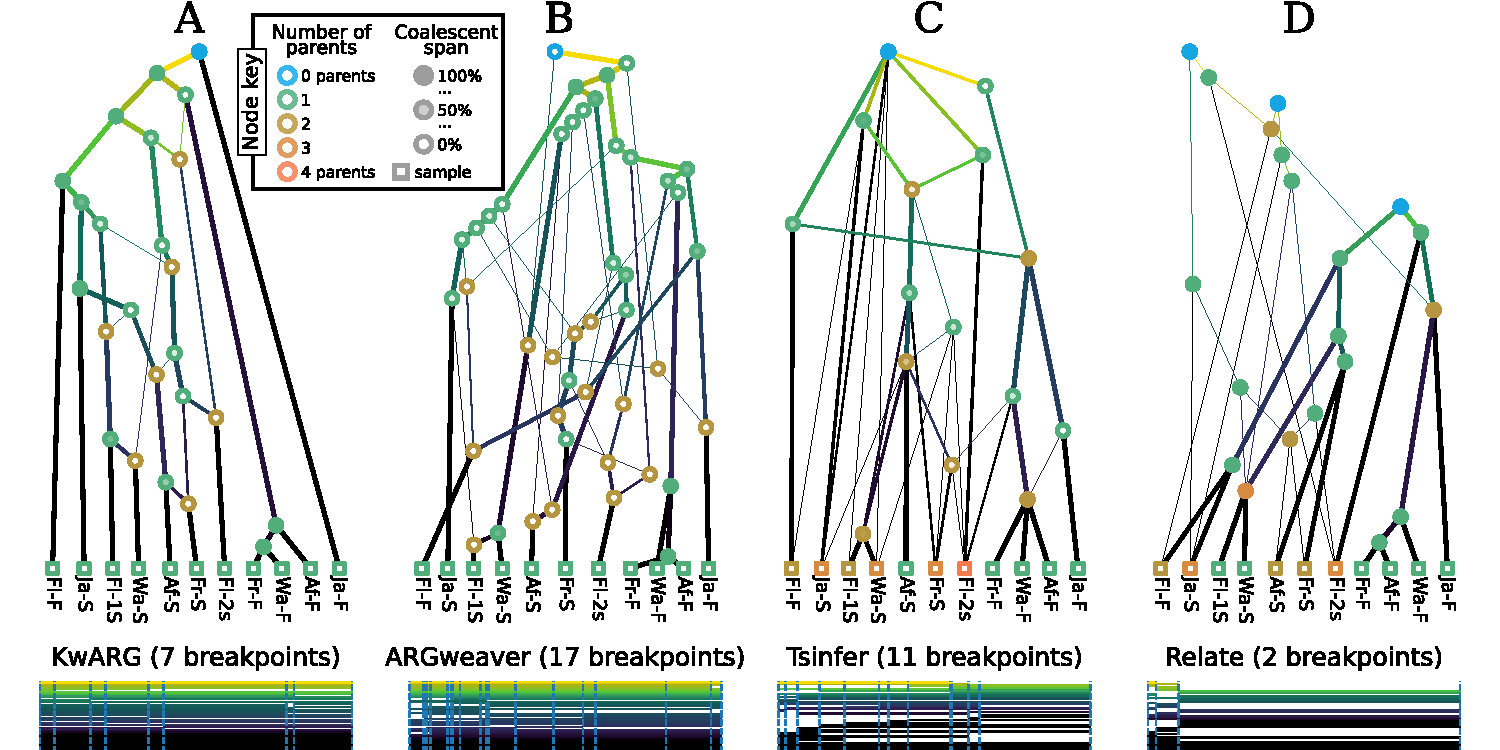
\includegraphics[width=\textwidth]{illustrations/inference.pdf} \end{center}
\caption{\label{fig-inferred-args} Inference results for
(A) \kwarg, (B) \argweaver, (C) \tsinfer,
and (D) \relate\
for 11 samples of a 2.7kb region of the \textit{Drosophila melanogaster} ADH
locus~\citep{kreitman1983nucleotide}.
The \argweaver\ example
is a sample from the inferred posterior distribution.
Edge colours are based on the time of the edge's child node
(lighter: older; darker: younger).
Position on the X and Y axes for the graph visualization is arbitrary.
Line width and node colour are as described in Fig.\ref{fig-simplification}.
The genomic intervals associated with edges are shown below
each ARG, where each row is an edge
and the X axis reflects genomic position.
Vertical lines indicate breakpoints between local trees.
}
\end{figure}

The example of successive simplification of a simulated ARG
in Fig.~\ref{fig-simplification} illustrates the point
that is is possible to \emph{store} arbitrary levels of precision
about recombination in a gARG.
It is also possible to \emph{infer} various levels of precision about
recombination.
To illustrate this, and to demonstrate the structural
heterogeneity of the ARGs inferred  by current methods,
Fig.~\ref{fig-inferred-args} shows the results of ARG inference
% To illustrate these points and to emphasise the heterogeneity
% of the ARGs inferred by current methods, we inferred ARGs for the
for the classical \citet{kreitman1983nucleotide} benchmark dataset
using  \kwarg~\citep{ignatieva2021kwarg},
\argweaver~\citep{rasmussen2014genome,hubisz2020inference},
\tsinfer~\citep{kelleher2019inferring},
and \relate~\citep{speidel2019method}.
% While there is some consistency among the inferred ARGs (such as the samples
% FR-F, WA-F and Af-F being grouped into the same clade), there
% are also considerable differences.
The minimum number
of recombination breakpoints required in the absence of recurrent mutation
is 7 for this dataset~\citep{song2003parsimonious},
and the number of inferred breakpoints
under the input mutation and recombination rates
varies from 2 (\relate) to 17 (\argweaver).
% TODO this needs a bit of rewriting with the rest of the paper in mind
% kwarg and argweaver are inferring eARGs, but we need to be careful
% not to confuse people.
The ARGs inferred by the different methods also have major differences
in how recombination information is represented.
Essentially,
\kwarg\ and \argweaver\ infer eARGs that contain
specific recombination \emph{events} for each breakpoint.
On the other hand, \tsinfer\ and
\relate\ do not infer events but rather
infer gARGs with by differing levels of precision about recombination.
The bottom row of Fig~\ref{fig-inferred-args} shows the extent along
the genome to which graph edges are shared between multiple trees.
We can see, for example, that the \relate\ trees ``share'' less topology
than other methods, but it certainly does not infer a series of
\emph{unrelated} local trees (i.e., with either unlabelled internal
nodes or differently labelled nodes in each tree).
The ARGs inferred by \relate\ and \tsinfer\ both contain substantial
information about node sharing across trees; for example,
both infer that Af-f, Fr-f and Wa-f share a common ancestor along
the entire sequence.
They contain a level of detail about recombination
that lies somewhere between a sequence of unrelated local trees on one
extreme and a completely precise event ARG on the other.

\section{Computational efficiency and data interchange}
\label{sec-efficiency}
ARG inference methods have been successfully applied to vast datasets,
including 500,000 genotyped humans~\citep{kelleher2019inferring,zhang2023biobank}
from UK Biobank~\citep{bycroft2018genome}
and over a million SARS-Cov-2 whole genomes~\citep{zhan2023towards}.
Even larger datasets are
available~\citep[e.g.][]{halldorsson2022sequences} % TODO more
and it seems inevitable that ARGs will be inferred for them.
The efficiency with which we can store and analyse these inferred
ARGs is therefore of great importance, and a key factor
in the ultimate success of downstream ARG-based methods.
Another key factor in how important ARG-based methods become
across the wide range of possible applications
% TODO more?
areas~\citep{rasmussen2014genome,harris2019database,
hejase2020summary,schaefer2021ancestral,
fan2022genealogical,wohns2022unified,harris2023using,
nowbandegani2023extremely,ignatieva2023distribution}
is how well inference methods and downstream analysis applications
interoperate. Without a well-defined and efficient shared format
for ARG data interchange,
users will suffer from problems with converting data from one program's
output to another, an unfortunate hallmark of population genetics
software for many years~\citep{excoffier2006computer}.
While current methods tend to tightly couple downstream analysis
of the inferred ARG with the inference
itself within the same software package,
this approach scales poorly in terms of software development
effort, and is ultimately not compatible with the widespread use
of ARGs for routine data analysis, and a healthy and diverse
software ecosystem.

The gARG encoding discussed and concretely defined in this manuscript
leads to highly efficient storage and processing of ARG data,
and has already been in use for several years.
The succinct tree sequence data structure (usually known as a ``tree sequence''
for brevity)
is a concrete encoding of a gARG, as discussed in this article.
It was originally developed as part of the \texttt{msprime}
simulator~\citep{kelleher2016efficient} and has subsequently been
extended and applied to forward-time
simulations~\citep{kelleher2018efficient,haller2018tree},
inference from data~\citep{kelleher2019inferring,wohns2022unified},
and calculation of population genetics statistics~\citep{ralph2020efficiently}.
The succinct tree sequence encoding extends the basic definition
of a gARG provided here by stipulating a
simple tabular representation and nodes and edges,
and also defining a concise and lossless representation of
sequence variation using the ``site'' and  ``mutation'' tables.
(Technically, edges in tree sequence terminology would be better
described as ``edge-intervals'', as each describes a single contiguous
interval of genome inheritance between a pair of nodes. This
denormalisation of the gARG data model in \texttt{tskit} is for efficiency purposes.)
The \texttt{tskit} library is a liberally
licensed open source toolkit that provides a comprehensive suite
of tools for working with gARGs (encoded as a succinct tree sequence).
Based on core functionality written
in C, it provides interfaces in C, Python and Rust.
Tskit is mature software, widely used in population genetics, and
has been incorporated into several downstream
applications~\citep[e.g.,][]{haller2019slim,speidel2019method,
adrion2020community,
terasaki2021geonomics,
baumdicker2021efficient,
fan2022genealogical,korfmann2022weak,
mahmoudi2022bayesian,petr2022slendr,rasmussen2022espalier,
zhang2023biobank,nowbandegani2023extremely,ignatieva2023distribution}.

% FIXME this needs more work and doesn't really fit into the
% narrative right now, but we do need to make this point.
The key insight that makes the succinct tree sequence encoding
an efficient substrate for defining analysis algorithms is that
it allows us to generate the local trees along the genome
in a way that allows us to reason about the \emph{differences}
between those trees.
Sequentially generating the local trees along the genome
is also fundamental, and is necessary whenever we need to
perform calculations that are contingent on more than just the
isolated properties of an edge. \cite{kelleher2016efficient}
showed how all trees can be sequentially generated in
constant time per tree transition in a fully simplified gARG.
Furthermore, we can easily reason about how tree topologies
change (and stay the same), leading to efficient algorithms
for computing population genetic
statistics~\citep{kelleher2016efficient,ralph2020efficiently},
implementing the Li and Stephens
model~\citep{kelleher2019inferring,wohns2022unified}
and likely many more.



% \cite{shipilina2023origin} discuss the idea of a ``haplotype block''
% (equivalent to the ``bricked tree sequence'' of
% \cite{nowbandegani2023extremely},
% % TODO look this up. I expect it's basically the same??
% and the block-based ARG data structure of
% \citep{palamara2016argon}),
% here we consider the unique sets of
% samples that coalesce at a node in the ARG over a particular
% genome interval, and the fundamental limitations they place
% on ARG inference.
% [FIXME find somewhere natural for this. The last clause is too vague - what
% are the implications?]
% Alternative gARG encodings split transmitted intervals and associate each with
% a new node, resulting in a single genome being represented by a group of
% multiple nodes (or ``blocks'' \citep{palamara2016argon}), with implications for

%%%% Some old text about the coalescent we might still want to plunder
% % If we want to use the coalescent, then really the assumptions
% % need to make sense.
% % n << Ne is a silly assumption in today's datasets
% A core assumption of the coalescent is that the sample size $n$
% is much less than the effective population size, $N_e$.
% Several human datasets now consist of hundreds of thousands of
% genomes~\citep{bycroft2018genome,karczewski2020mutational,tanjo2021practical},
% and so sample size is substantially \emph{larger} than $N_e$
% (often assumed to be $10^4$ in humans).
% Agricultural datasets are even more extreme.
% For example,
% the US dairy cattle database alone currently comprises more than 6 million
% animals with SNP array
% genotypes\footnote{\url{https://queries.uscdcb.com/Genotype/counts.html}},
% while the effective population size in modern dairy cattle breeds is
% less than 100 and decreasing~\citep{MacLeod2013,Makanjuola2020}.
% An extreme sign of these breeding practices is that there are only two ancestral
% Y-chromosome lineages present in today's US Holstein dairy breed~\citep{Yue2015}.
% Simlarly, the 1000 bull genomes project~\citep{hayes20191000}
% comprises close to 7000 genomes, which are part of multi-generation pedigrees
% with millions of animals and extensive SNP array genotype and phenotype
% data \citep[e.g.][]{Cesarani2022}.
% In another example, genome and SNP array data for 440,610 individuals within
% 7 multi-generation pedigrees~\citep{whalen2018,Johnsson2021,Ros-Freixedes2020}
% were combined to infer recombination in pigs~\citep{RosFreixedes2022}.
% Effective population size in modern pig breeds is also less than 100 due to
% intense selection and directed reproduction \citep{Hall2016,Porcnic2016}.
% Another core assumption of the coalescent model is that the genome (or
% at least the region under study) is short enough that the number of extant
% lineages remains much smaller than $N_e$ at all times. Whole
% genome sequences have been available for model organisms
% for over a decade now, % True? Citation?
% and indeed complete chromosome-level assemblies are possible
% in humans~\citep{miga2020telomere}.
% Projects are under way to obtain high-quality assemblies
% for all eukaryotic species in Britain and Ireland~\citep{darwin2022sequence}
% and ultimately worldwide~\citep{lewin2022earth}.

\section{Discussion}
\label{sec-discussion}
Recent breakthroughs have finally made large-scale ARG inference
feasible in practice, leading to a surge of interest
in development of ARG-based inference methods, their evaluation
and application.
The prospect of ARGs being used routinely within population
and statistical genetics is tantalising,
but in reality there is substantial work to be done to
enable this.
A necessary first step is a degree of terminological clarity.
As discussed in Appendix~\ref{sec-arg-history}, the term
``ancestral recombination graph" has several
subtly different interpretations, depending on context.
The trend to decouple ARGs from their original definition
within the context of stochastic
processes and instead use the term as a more general representation of any
recombinant genetic ancestry seems useful, and we have
tried to clarify and systematise it here. Thus
we can think of an ARG as any structure that encodes the
reticulate genetic ancestry of a sample of colinear sequences under
the influence of recombination. The ``genome'' ARG (gARG) encoding
made explicit here is one way we can concretely
define such recombinant ancestry, which we have shown is both
flexible and efficient.
The flexibility of the gARG encoding contrasts with the classical
``event'' ARG (eARG), which is more limited in what can be described, because of its origins in an idealised mathematical model.

Fully decoupling the general concept of an ARG from the coalescent
with recombination stochastic process is an important step.
While this has proven to be a useful and
robust
model~\citep{wakeley2012gene,bhaskar2014distortion,nelson2020accounting},
many modern datasets have properties that grossly
violate its assumptions.
For instance, several human datasets now consist of hundreds of thousands of
% TODO cite GeL paper
genomes~\citep{bycroft2018genome,karczewski2020mutational,tanjo2021practical},
and so sample size is substantially \emph{larger} than the
usually assumed $N_e$ values.
Agricultural datasets are an even more extreme departure from coalescent
assumptions, with hundreds of thousands of samples embedded in
multi-generational pedigrees~\citep{hayes20191000,Ros-Freixedes2020}
and effective population sizes of 100 and even
less~\citep{MacLeod2013,Makanjuola2020,Hall2016,Porcnic2016}.
Even if sufficiently complex demographic models~\citep{gower2022demes}
encompassing hundreds of populations, explosive growth rates and
myriad interconnections of migration, were somehow estimated and
provided as input, ARGs sampled from
the coalescent cannot capture the complexities of realistic family structures, which often involve overlapping generations and extreme variation in lifetime reproductive success. Flexible ARG encoding should accommodate such cases.

Given that there is no single model that can capture the complexities
of modern datasets across species (and taxa; see discussion of SARS-CoV-2
below), we cannot rely on sampling from a distribution to capture
the uncertainty in our ARG estimates. Indeed, even if the coalescent
were a suitable model for datasets such as UKB and we had a means of
sampling from its distribution of ARGs at the scale of hundreds of thousands
of samples, we could only explore the tiniest corner of such an incomprehensibly
large space of possibilities.
Therefore, it is important to systematically
describe and utilise uncertainty about ARG inference.
One approach, enabled by the gARG encoding described here, is to allow
nodes to have (rootward) in-degree greater than two (polytomies
representing uncertainty over the ordering of coalescence events) or
out-degree greater than two (representing uncertainty over the ordering
of multiple recombination events). Development of other methods to capture, for example,
uncertainty about node ages and recombination breakpoint positions, is an important
aspect of future work.

The timing, positions, and even the number of recombination events is generally
not possible to infer precisely from genome sequencing data. For ARGs under
coalescent-based models, the proportion of recombination events that change the
ARG topology grows very slowly with sample size \citep{hein2004gene}, and of those
events only a small proportion are actually detectable from the data, assuming
human-like mutation rates \citep{myers2002detection,hayman2023recoverability}.
Even when a recombination event \emph{is} detectable, its timing and breakpoint
positions can only be inferred approximately, depending on how much information
can be elucidated from mutations in the surrounding genomic region. For general
ARGs, for instance those representing pedigrees, or genealogies of organisms with
low mutation rates and complex patterns of recombination, such inference can be
even more challenging. The fact that the eARG encoding \emph{requires}
precise estimates about recombination is therefore a fundamental limitation, which
is a central message of this paper.
% This might be where we mention Fisher's junctions and IBD?
% https://github.com/tskit-dev/what-is-an-arg-paper/issues/121

% % Do downstream applications actually make use of such full ARGs?
Besides the inherent limitations that exist on inferring fully
precise ARGs from data,
we should also consider the value that such precise estimates provide
for downstream applications.
To date, few downstream applications using estimated ARGs
make use of complete recombination information.
Most applications work by examining local trees independently.
For example, the \relate\ selection test~\citep{speidel2019method}
obtains $p$-values by computing clade size probabilities conditional on the timing of coalescence events in a given local tree.
In their method
for estimating dispersal rates and the locations of genetic
ancestors,
\citep{osmond2021estimating} downsample trees along the genome
so that they can be regarded as approximately independent.
The SIA method for detecting selection~\citep{hejase2022deep}
encodes local trees as a set of lineage counts at discrete
time intervals, and uses these as feature for a
type of machine learning algorithm
that takes ``temporal'' correlations into account. Thus,
while SIA does use some of the information about local tree correlation,
clearly much of the detail about recombination
events in an ARG is lost.
The \texttt{tsdate} algorithm (and related naive estimator
of ancestral location) uses much more between-tree
information~\citep{wohns2022unified}, explicitly using the gARG
encoding to reason about ancestral nodes.
The main application for fully precise ARGs thus far has been
to compute a likelihood under the coalescent with
recombination~\citep[e.g.][]{kuhner2000maximum,mahmoudi2022bayesian},
which currently requires the details of all recombination
events to be known.

% Note: haven't said anything about the coalescent here. Do we need to?
The advantages of a model-agnostic representation that naturally
incorporates uncertainty about the ordering of events in an ARG are well-illustrated by~\cite{zhan2023towards}, who
inferred ARGs using millions of SARS-CoV-2 sequences from the
GISAID database~\citep{shu2017gisaid}. In contrast to typical human sequencing datasets, the SARS-CoV-2 data is
sampled continuously through time, sometimes with tens of thousands of sequences collected per day, with relatively little genetic diversity to
distinguish them. The reconstructed ARGs thus contain polytomies (representing
both the uncertainty around coalescence times and the presence of true
multiple mergers), non-leaf sample nodes (sequences with descendants
also present in the dataset) and unary nodes (samples that have
one other sampled descendant). Recombination is known
to be an important factor in the evolution of SARS-CoV-2~\citep{vaninsberghe2021recombinant,jackson2021generation,ignatieva2022ongoing},
and the ARGs also contain recombination nodes.
Because parental sequences
are generally never sampled themselves, and often
a recombinant strain is the product of multiple recombination events,
uncertainty around this is captured by recording the ancestry
of each part of the recombinant sequence without arbitrarily assigning
times or orderings for these events. This demonstrates the flexibility of the gARG
encoding in capturing recombinant genealogies regardless of the underlying
(possibly unknowable) generative evolutionary process.

This view of ARGs,
decoupled from generative models and
without the hard requirement
of complete precision on all historical events, may clarify inference goals and improve
methods for evaluation.
In most cases,
ARG inference is evaluated by simulating data from a known ground truth ARG,
and comparing this to the inferred version via pairwise comparison of
local trees along the genome, for example
using tree distance
metrics~\citep[e.g.][]{robinson1981comparison,kendall2016mapping},
as described by \citet{kuhner2015assessing}.
% While this provides valuable insights into the method's performance,
% it is not clear how well these tree distance metrics reflect
% performance on real data.
In comparing tree-by-tree along the genome, the effects of recombination
are only incorporated in an indirect manner through the correlations
between the local trees, rather than through directly taking into account
the persistence of nodes and edges across multiple trees.
The performance of tree distance metrics varies by
application~\citep{kuhner2015assessing}, and the correct approach
to handling subtleties such as polytomies
is an open question~\citep{kelleher2019inferring,zhang2023biobank}.
% Is this true? These guys claim RF takes linear time:
% https://bmcgenomics.biomedcentral.com/articles/10.1186/s12864-020-07011-0
Tree distance metrics usually have at least $O(n^2)$ time complexity
and therefore cannot be
applied to the very large sample sizes currently of interest.
A recent trend has been to move away from such
tree distance-based approaches and to examine more properties of the inferred ARGs.
\citet{brandt2021evaluation} focussed on the
distributions of pairwise MRCA times;
\citet{deng2021distribution} derived an approximation to the distribution of the
waiting distances between local trees;
\citet{ignatieva2023distribution}
derived the distribution of the genomic span of an edge and that of a
clade of samples. In each case, simulation studies demonstrated
substantial differences between these quantities in simulated and reconstructed ARGs,
that were not captured using tree-by-tree comparisons.
% Not sure this is the right place for this sentence
These evaluations have been based on
ground truth data from highly idealised simulations, with sample sizes limited to at most a few thousand (typically much fewer).
The effects of the richness of real data
on modern biobank-scale or multi-generational pedigree datasets
are almost entirely unknown (beyond studies using very simplistic error models).
The development of ARG evaluation metrics that take into account more of the
global topology and can be applied to large ARGs would be a
valuable and timely addition to the field.

Interest in ARG inference methods and downstream applications is
burgeoning, with exciting developments arriving at ever-increasing pace.
Without agreement on basic terminology and some standardisation
on data formats, however, the ARG revolution may falter.
Here, we have advocated
for decoupling the data structures used to represent ARGs
from generative processes, and have shown that the
gARG encoding enables flexible description of
contemporary datasets with varying levels of precision and integral
handling of some important forms of temporal uncertainty.
For ARG-based methods to achieve mainstream status, we require
a rich supporting software ecosystem.
Ideally, this would comprise a wide range of different
inference methods specialised to different organisms, types
and scales of data and
% I'm thinking about things like Espalier specifically wanting
% to characterise the recombs, vs Relate mainly wanting to
% get good local trees
specific inference goals, sharing a common ARG interchange format.
The output of these diverse inference methods could then be
processed by numerous downstream applications,
enabling users to freely compare the outputs of different
inference methods on their data, and the result of different
analyses on these inferences.
Earlier efforts to standardise ARG interchange shared
this vision,
but did not succeed~\citep{cardona2008extended,mcgill2013graphml}.
Today, however, we have the benefit of a pre-existing ARG
interchange format, already widely used and accompanied
by high-quality, high-performance software
(see Section~\ref{sec-efficiency} for details).
Adopting the \texttt{tskit} library
as a community standard,
utilising its rich suite of operations,
may accelerate progress and help to
establish ARG methods within mainstream genetics.

\section*{Acknowledgements}
We are grateful to Nick Barton, Gideon Bradburd, Alex Lewanski and Andrew Vaughan
for helpful discussions and comments on the manuscript.

% Ordered alphabetically by surname
Gregor Gorjanc acknowledges support from the BBSRC ISP grant to The Roslin Institute (BBS/E/D/30002275, BBS/E/RL/230001A, and BBS/E/RL/230001C).
% Anastasia Ignatieva acknowledges support from TODO
Jerome Kelleher acknowledges support from the Robertson Foundation.
Jere Koskela acknowledges support from EPSRC research grant EP/V049208/1.
% Anthony Wilder Wohns acknowledges support from TODO

\bibliographystyle{plainnat}
\bibliography{paper}

\setcounter{secnumdepth}{2} % Print out appendix section numbers

% TODO revisit number here
\section*{Appendix}
\appendix

\setcounter{table}{0}
\setcounter{figure}{0}
\renewcommand{\thetable}{A\arabic{table}}
\renewcommand{\thefigure}{A\arabic{figure}}

\section{Ancestral graphs: a brief history}
\label{sec-arg-history}
The coalescent~\citep{kingman1982coalescent,kingman1982genealogy,
hudson1983testing, tajima1983evolutionary} models the ancestry of a sample of
genomes under an idealised population model, and provides the theoretical
underpinning for much of contemporary population genetics.
It is a stochastic process, where each random realisation
is a genealogical tree describing the genetic ancestry of the sample.
Numerous extensions to the model have been
proposed~\citep{hudson1990gene,hein2004gene,wakely2008coalescent},
incorporating many evolutionary processes.
\citet{hudson1983properties}
first incorporated recombination into the coalescent process,
providing several fundamental analytical results
and describing the basic simulation algorithm, still in
widespread use~\citep{hudson2002generating,kelleher2016efficient,
baumdicker2021efficient}.
In the 1990s, Griffiths and colleagues revisited the
coalescent with recombination from a different perspective,
formulating it as a stochastic process where each realisation
is encoded as a graph~\citep{griffiths1991two,ethier1990two,
griffiths1996ancestral,griffiths1997ancestral}.
They referred to both the stochastic process and
its random realisations as the Ancestral Recombination Graph (ARG).
Although mathematically equivalent, it is
important to note that the Griffiths and Hudson formulations of
the coalescent with recombination are not identical;
in particular, a direct implementation of the ARG process
as originally described requires exponential time to simulate
(see Appendix~\ref{big-and-little-arg} for details). However, ARGs provided a way
to reason about and infer recombinant ancestry as a single object,
which was not possible within Hudson's framework, which emphasised
the collection of local trees along the genome resulting from recombination.

Subsequent work on ARGs proceeded in broadly three main directions: focussing on (1)
exploring the mathematical properties of the coalescent with recombination and
related stochastic processes, (2) inferring evolutionary parameters under
(approximations to) this model, either with or without explicitly reconstructing the
genealogy of the sample, and (3) treating the ARG as a discrete graph, ignoring the
generating stochastic process, and studying its properties from a computational and
algorithmic perspective.

% Mathematical treatment of the CwR and ARGs (and ARG-like stochastic processes)
An extensive body of work has been developed from
studying the coalescent with recombination
% Can we add a couple of the most well known CwR examples here
and other related
graph-valued stochastic processes from a mathematical perspective.
In particular, the Ancestral Selection Graph
(ASG)~\citep{krone1997ancestral,neuhauser1997genealogy}
uses a similar approach to model natural selection instead of recombination.
Unlike the ARG process, the ASG imposes a hard distinction between the stochastic process,
which constructs a random ARG-like graph, and an observable realisation,
which is a single tree sampled from the graph in a non-uniform way to encode
desired patterns of natural selection.
Constructions of ASG-like stochastic processes encoding various
forms of selection, often in parallel with recombination or other genetic forces,
are an area of considerable and ongoing theoretical interest~\citep[e.g.][]{
neuhauser1999ancestral,
donnelly1999genealogical,
fearnhead2001perfect,
fearnhead2003ancestral,
etheridge2009coalescent,
gonzalezcasanova2018duality,
koskela2019robust}.
% Could mention the Ancestral Gene Transfer graph here too, within
% something like "Similarly the Ancestral Gene Transfer Graph [cite]
% and [other ancestral graphs, if they exist?] model genealogical
% processes in bacteria as a graph.

% Inference of parameters and explicit ARG reconstruction
Early work on inference under the coalescent with recombination
focused on the problem of
inferring the parameters of the
stochastic process, where the ancestry was regarded as a
latent parameter to be averaged out
\citep[e.g.][]{griffiths1996ancestral,kuhner2000maximum, nielsen2000estimation,
fearnhead2001estimating}.
These methods met with limited success
because the state space of ARGs is overwhelmingly large, and
lacks a simple geometry or neighbourhood structure for inference or
sampling methods to  exploit.
Several breakthroughs in this direction were achieved through
formulating simplified but more tractable approximations to the full
model~\citep{mcvean2005approximating,marjoram2006fast,li2011inference,
paul2011accurate,schiffels2014inferring}.
The related problem of \emph{sampling} genealogies compatible with a given
dataset under the coalescent with recombination also proved notoriously difficult
computationally; progress in explicitly inferring genealogies at scale
has similarly been achieved through resorting to principled
approximations~\citep{rasmussen2014genome,mahmoudi2022bayesian},
or moving away from the coalescent with recombination altogether and seeking
to infer a single plausible ARG~\citep[e.g.][]{speidel2019method} or ARG
topology~\citep[e.g.][]{minichiello2006mapping,kelleher2019inferring}.

% Optimisation problems to do with ARGs and other phylogenetic networks
There has also been substantial interest in formulating and answering
fundamental questions about properties
of the ARG as a discrete graph structure, focusing on the ARG topology without considering
either branch lengths or indeed the generating process.
The first prominent problem was calculating (lower bounds on) the minimum number of
recombinations required to reconstruct a valid genealogy for a given
sample~\citep{myers2003bounds}, and constructing the corresponding
minimal (parsimonious)
ARGs~\citep{song2003parsimonious,song2005efficient,lyngso2005minimum}.
These problems are NP-hard in general~\citep{wang2001perfect}, and progress has
been achieved through studying various constrained special cases of ARGs~\citep[e.g.][]{gusfield2004optimal} and
other more general types of phylogenetic networks~\citep{huson2010phylogenetic}. The
focus has been on algorithmic and combinatorial results~\citep{gusfield2014recombinatorics}
that are often not of
direct relevance to the inference problems described above.

%It is important to note that parsimonious ARGs
%have quite different properties from realisations of the
%ARG \emph{process} as modelled by Hudson, Griffiths, and colleagues.
%Firstly, branch lengths are not typically estimated,
%% why do we need the following two lines
%and node times are required in order to compute a likelihood under the
%coalescent with recombination (see section XXX).
%Secondly, even if branch lengths were estimated,
%the realisations would have a very small likelihood since
%the coalescent with recombination is often highly \emph{un}parsimonious
%in terms of recombination events.

The goal of this historical overview is to illustrate that the meaning of the term ``ARG" now strongly
depends on the context in which it is used, and can mean both the
stochastic process that generates genealogies in the presence of
recombination~\citep[e.g.][]{nordborg2000linkage,birkner2013ancestral,
wilton2015smc,griffiths2016coalescent},
as well as, more commonly, the concrete realisation of ancestry from a
process~\citep[e.g.][]{gusfield2014recombinatorics,mathieson2020ancestry,brandt2021evaluation}.
\cite{minichiello2006mapping} explicitly distinguished the ARG as a
stochastic process from the ARG as a data structure. We have followed them and
used the term in the latter sense, to mean a specific realised ancestral history.

\section{The Big and Little ARG}
\label{sec-big-and-little-arg}
Here we review the two predominant stochastic processes which construct ARGs:
the ``big" ARG process of \cite{griffiths1997ancestral}, and the ``little" ARG process of
 \cite{hudson1983properties}. The big ARG process is mathematically simpler
 but is computationally intractable due to generating a vast number of ancestors
 which contribute no genetic material to the initial sample.
The little ARG process avoids non-genetic ancestors at the cost of more complex
dynamics and state space. We also demonstrate that evaluating the sampling probability
of either process---a key quantity in many statistical approaches---requires that the
gARG (or eARG) data structure be interpreted in a model-specific way.

A generic state of the little ARG process consists of a finite collection of lineages $L$,
each of which is a list of disjoint ancestry segments $(\ell, r, a)$, where
$[\ell, r)$ is a half-closed genomic interval and $a$ is an integer
tracking the number of samples to which the lineage is ancestral over that interval.
We also usually track the node associated with each segment, but
that is not important for our purposes here so we omit it to lighten notation.
The initial condition for a sample of $n$ genomes of length $m$ consists of $n$ lineages
of the form $\{(0, m, 1)\}$. The process traverses a series of common ancestor and
recombination events backwards in time.
Recombination events happen at rate $\rho \nu / (m - 1)$,
where $\rho \geq 0$ is a per-genome recombination rate and
 \[
 \nu = \sum_{x \in L}\left( \max_{(\ell, r, a) \in x}r
     - \min_{(\ell, r, a) \in x}\ell - 1 \right)
 \]
 is the number of available ``links" surrounded by ancestral material.
 At a recombination event we choose one of these links uniformly and break it,
 replacing the original lineage in $L$ with two new lineages containing the ancestral material
 to the left and right of the break point, respectively.

Common ancestor events occur at rate $\binom{|L|}{2}$.
In a common ancestor event, two uniformly sampled lineages have their segments
merged into a single ancestor lineage, which is added to $L$.
If the lineages have overlapping intervals of ancestry,
say, $(\ell, r, a_1)$ and $(\ell, r, a_2)$, a
\emph{coalescence} occurs. The result is a segment
$(\ell, r, a_1 + a_2)$, and if $a_1 + a_2 < n$ it is included in the
ancestor lineage. Otherwise, if $a_1 + a_2 = n$, we have found
the most recent common ancestor of all samples in the interval $[\ell, r)$
and do not need to simulate its history any further.
Non-overlapping intervals from the two lineages are included
 in the ancestor lineage without changes. Eventually,
we find resultant lineages in which all segments have fully coalesced,
and so the number of extant lineages gradually falls to zero.

In the Griffiths formulation (the big ARG process), each edge in the graph corresponds to an extant
lineage and nodes are events in the process. The $n$ initial leaf nodes are
sampling events. Common ancestor events occur at rate $\binom{|L|}{2}$.
When a common ancestor event happens, two uniformly chosen lineages
merge into a common ancestor lineage.
Recombination events happen at rate $|L| \rho$. Here, we choose a lineage (i.e.\ edge) uniformly,
and a breakpoint $0 < x < m$ uniformly on its genome. We terminate the edge at a
node, record the breakpoint, and start two new edges from this node. The process
then continues until there is only one lineage left (the Grand Most Recent
Common Ancestor, GMRCA), which is guaranteed to
happen in finite time because of the quadratic rate of coalescing vs.\ linear rate of branching.

The state-space of the big ARG process is much simpler than that of the little ARG process,
which greatly facilitates mathematical reasoning. This simplicity comes at a
substantial cost, however, if we wish to use it as a practical means of
simulating recombinant ancestries.
The number of events in the big ARG all the way back to the GMRCA
is $O(e^\rho)$~\citep{griffiths1997ancestral}, whereas the number
of events required to simulate the little ARG is
$O(\rho^2)$~\citep{hein2004gene,baumdicker2021efficient}.
This disparity arises because the majority of the events in the big ARG are
recombination events which occur outside of ancestral material,
and this do not have any bearing on the ancestry of the initial sample.
Because we don't keep track of the distribution of ancestral material during the process,
we generate a vastly larger graph.

Figure \ref{hudson_vs_bigARG} illustrates the more complex state space
of the little ARG process, as well as the extra events which occur in the big ARG process.
Moreover, it depicts the rates of common ancestors and recombination events in each
interval of time of the realisations.
In order to evaluate these rates, and hence the sampling probability
\cite[see e.g.][Equation (3)]{mahmoudi2022bayesian},
it is necessary to know the number of lineages and number of extant links
available for recombination in each time interval.
Some representations may not provide this information.
For example, in the gARG encoding depicted in Figure \ref{fig-ancestry-resolution}C
it is clear that a recombination takes place between nodes \noderef{b} and
\noderef{d} as well as \noderef{e}, but the exact time of the event is ambiguous,
and thus so is the number of lineages during the time interval. In fact, this
information cannot be recovered from the gARG encoding used in Figure \ref{fig-ancestry-resolution}C,
and alternative conventions must be introduced to resolve such ambiguities.
For the likelihood-based inference algorithms for the coalescent with recombination,
it is sufficient to create \emph{two} gARG nodes at the time of the recombination event:
see the appendix of \cite{baumdicker2021efficient} for details of evaluating
coalescent with recombination likelihoods using this convention.
This is also the interpretation depicted in
Figure \ref{hudson_vs_bigARG}, but it means that the two edges above node \noderef{b}
in Figure \ref{fig-ancestry-resolution} should correspond to only one lineage,
along which all $m-1$ links are available for recombination.
The lineage then splits into two at the time of nodes \noderef{d} and \noderef{e}.
Nodes \noderef{k}, \noderef{l}, and \noderef{m} in Figure \ref{fig-ancestry-resolution}
demonstrate that the same issue can affect the number of links available for recombination:
without an external convention, the exact time at which the trapped ancestral material on
node \noderef{k} ceases to be available for an effective recombination in the little ARG process.

\begin{figure}[t]
\centering
% FIXME this is a quick nasty hack to make the figure a bit smaller and
% prevent flushing all the other figures to the end of the document.
\scalebox{0.54}{
\begin{tabular}{cc}
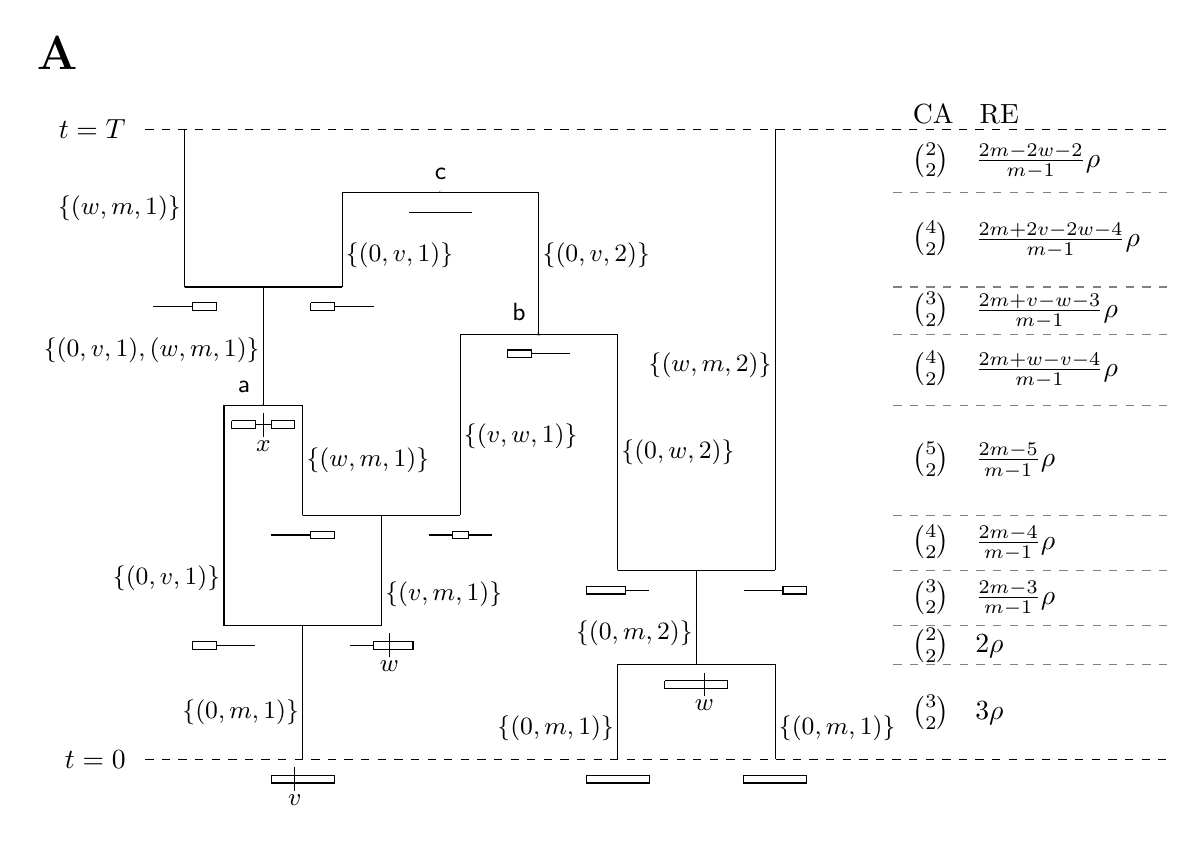
\begin{tikzpicture}
	\node [anchor=north west] at (-3.5,9.3) {\LARGE \textbf{A}};
	\draw (-0.4, -0.2) -- (0.4, -0.2) -- (0.4, -0.3) -- (-0.4, -0.3) -- (-0.4, -0.2);
	\draw (-0.1, -0.1) -- (-0.1, -0.4);
	\node [label=below:{\small $v$}] at (-0.1, -0.2) {};
	\draw (3.6, -0.2) -- (4.4, -0.2) -- (4.4, -0.3) -- (3.6, -0.3) -- (3.6, -0.2);
	\draw (5.6, -0.2) -- (6.4, -0.2) -- (6.4, -0.3) -- (5.6, -0.3) -- (5.6, -0.2);

	\draw (4,0) -- (4, 1.2) -- (6, 1.2) -- (6,0);
	\draw (4.6, 1) -- (5.4, 1) -- (5.4, 0.9) -- (4.6, 0.9) -- (4.6, 1);
	\draw (5.1, 1.1) -- (5.1, 0.8);
	\node [label=below:{\small $w$}] at (5.1, 1) {};

	\draw (0, 0) -- (0, 1.7) -- (-1,1.7) -- (1,1.7);
	\draw (-1.4, 1.5) -- (-1.1, 1.5) -- (-1.1, 1.4) -- (-1.4, 1.4) -- (-1.4, 1.5);
	\draw (-1.1, 1.45) -- (-0.6, 1.45);
	\draw (0.6, 1.45) -- (0.9, 1.45);
	\draw (0.9, 1.5) -- (1.4, 1.5) -- (1.4, 1.4) -- (0.9, 1.4) -- (0.9, 1.5);
	\draw (1.1, 1.6) -- (1.1, 1.3);
	\node [label=below:{\small $w$}] at (1.1, 1.5) {};

	\draw (5, 1.2) -- (5, 2.4) -- (4,2.4) -- (6,2.4);
	\draw (3.6, 2.2) -- (4.1, 2.2) -- (4.1, 2.1) -- (3.6, 2.1) -- (3.6, 2.2);
	\draw (4.1, 2.15) -- (4.4, 2.15);
	\draw (5.6, 2.15) -- (6.1, 2.15);
	\draw (6.1, 2.2) -- (6.4, 2.2) -- (6.4, 2.1) -- (6.1, 2.1) -- (6.1, 2.2);

	\draw (1, 1.7) -- (1, 3.1) -- (0,3.1) -- (2,3.1);
	\draw (-0.4, 2.85) -- (0.1, 2.85);
	\draw (0.1, 2.9) -- (0.4, 2.9) -- (0.4, 2.8) -- (0.1, 2.8) -- (0.1, 2.9);
	\draw (1.6, 2.85) -- (1.9, 2.85);
	\draw (1.9, 2.9) -- (2.1, 2.9) -- (2.1, 2.8) -- (1.9, 2.8) -- (1.9, 2.9);
	\draw (2.1, 2.85) -- (2.4, 2.85);

	\draw (-1, 1.7) -- (-1, 4.5) -- (0,4.5) -- (0,3.1);
	\node [scale=0.2,label=above left:{\small \noderef{a}}] at (-0.5,4.5) {a};
	\draw (-0.9, 4.3) -- (-0.6, 4.3) -- (-0.6, 4.2) -- (-0.9, 4.2) -- (-0.9, 4.3);
	\draw (-0.6, 4.25) -- (-0.4, 4.25);
	\draw (-0.4, 4.3) -- (-0.1, 4.3) -- (-0.1, 4.2) -- (-0.4, 4.2) -- (-0.4, 4.3);
	\draw (-0.5, 4.4) -- (-0.5, 4.1);
	\node [label=below:{\small $x$}] at (-0.5, 4.3) {};

	\draw (4,2.4) -- (4,5.4) -- (2,5.4) -- (2,3.1);
	\node [scale=0.2,label=above left:{\small \noderef{b}}] at (3,5.4) {b};
	\draw (2.6, 5.2) -- (2.9, 5.2) -- (2.9, 5.1) -- (2.6, 5.1) -- (2.6, 5.2);
	\draw (2.9, 5.15) -- (3.4, 5.15);

	\draw (-0.5, 4.5) -- (-0.5, 6) -- (-1.5,6) -- (0.5,6);
	\draw (-1.9, 5.75) -- (-1.4, 5.75);
	\draw (-1.4, 5.8) -- (-1.1, 5.8) -- (-1.1, 5.7) -- (-1.4, 5.7) -- (-1.4, 5.8);
	\draw (0.1, 5.8) -- (0.4, 5.8) -- (0.4, 5.7) -- (0.1, 5.7) -- (0.1, 5.8);
	\draw (0.4, 5.75) -- (0.9, 5.75);

	\draw (0.5, 6) -- (0.5, 7.2) -- (3,7.2) -- (3,5.4);
	\node [scale=0.2,label=above:{\small \noderef{c}}] at (1.75,7.2) {c};
	\draw (1.35, 6.95) -- (2.15, 6.95);

	\draw (-1.5, 6) -- (-1.5, 8);
	\draw (6, 2.4) -- (6, 8);

	% Edge annotations above each event
	\node [label=left:{\small$\{(0,m,1)\}$}] at (0.2,0.6) {};
	\node [label=left:{\small$\{(0,m,1)\}$}] at (4.2,0.4) {};
	\node [label=right:{\small$\{(0,m,1)\}$}] at (5.8,0.4) {};
	\node [label=left:{\small$\{(0,m,2)\}$}] at (5.2,1.6) {};
	\node [label=left:{\small$\{(0,v,1)\}$}] at (-0.8,2.3) {};
	\node [label=right:{\small$\{(v,m,1)\}$}] at (0.8,2.1) {};
	\node [label=right:{\small$\{(0,w,2)\}$}] at (3.8,3.9) {};
	\node [label=left:{\small$\{(w,m,2)\}$}] at (6.2,5) {};
	\node [label=right:{\small$\{(w,m,1)\}$}] at (-0.2,3.8) {};
	\node [label=right:{\small$\{(v,w,1)\}$}] at (1.8,4.1) {};
	\node [label=left:{\small$\{(0,v,1), (w,m,1)\}$}] at (-0.3,5.2) {};
	\node [label=right:{\small$\{(0,v,2)\}$}] at (2.8,6.4) {};
	\node [label=left:{\small$\{(w,m,1)\}$}] at (-1.3,7) {};
	\node [label=right:{\small$\{(0,v,1)\}$}] at (0.3,6.4) {};

	% Dashed lines for start and end times
	\draw[dashed] (-2, 0) -- (11, 0);
	\node [label=left:{$t = 0$}] at (-2,0) {};
	\draw[dashed] (-2, 8) -- (11, 8);
	\node [label=left:{$t = T$}] at (-2,8) {};

	% Numbers of extant ancestors and links, from top to bottom
	\node[label=right:{CA \; RE}] at (7.5, 8.2) {};
	\node[label=right:{$\binom{2}{2}$ \; $\frac{2 m - 2 w - 2}{m - 1} \rho$}] at (7.5, 7.6) {};
	\node[label=right:{$\binom{4}{2}$ \; $\frac{2 m + 2 v - 2 w - 4}{m - 1} \rho$}] at (7.5, 6.6) {};
	\node[label=right:{$\binom{3}{2}$ \; $\frac{2 m + v - w - 3}{m - 1} \rho$}] at (7.5, 5.7) {};
	\node[label=right:{$\binom{4}{2}$ \; $\frac{2 m + w - v - 4}{m - 1} \rho$}] at (7.5, 4.95) {};
	\node[label=right:{$\binom{5}{2}$ \; $\frac{2 m - 5}{m - 1} \rho$}] at (7.5, 3.8) {};
	\node[label=right:{$\binom{4}{2}$ \; $\frac{2 m - 4}{m -1} \rho$}] at (7.5, 2.75) {};
	\node[label=right:{$\binom{3}{2}$ \; $\frac{2 m - 3}{m - 1} \rho$}] at (7.5, 2.05) {};
	\node[label=right:{$\binom{2}{2}$ \; $2 \rho$}] at (7.5, 1.45) {};
	\node[label=right:{$\binom{3}{2}$ \; $3 \rho$}] at (7.5, 0.6) {};

	% Gray dashed lines to visually separate holding times
	\draw[color=gray, dashed] (7.5, 1.2) -- (11, 1.2);
	\draw[color=gray, dashed] (7.5, 1.7) -- (11, 1.7);
	\draw[color=gray, dashed] (7.5, 2.4) -- (11, 2.4);
	\draw[color=gray, dashed] (7.5, 3.1) -- (11, 3.1);
	\draw[color=gray, dashed] (7.5, 4.5) -- (11, 4.5);
	\draw[color=gray, dashed] (7.5, 5.4) -- (11, 5.4);
	\draw[color=gray, dashed] (7.5, 6) -- (11, 6);
	\draw[color=gray, dashed] (7.5, 7.2) -- (11, 7.2);
\end{tikzpicture}
&
\begin{tikzpicture}
	\node [anchor=north west] at (-3.5,9.3) {\LARGE \textbf{B}};
	\draw (-0.4, -0.2) -- (0.4, -0.2) -- (0.4, -0.3) -- (-0.4, -0.3) -- (-0.4, -0.2);
	\draw (-0.1, -0.1) -- (-0.1, -0.4);
	\node [label=below:{\small $v$}] at (-0.1, -0.2) {};
	\draw (3.6, -0.2) -- (4.4, -0.2) -- (4.4, -0.3) -- (3.6, -0.3) -- (3.6, -0.2);
	\draw (5.6, -0.2) -- (6.4, -0.2) -- (6.4, -0.3) -- (5.6, -0.3) -- (5.6, -0.2);

	\draw (4,0) -- (4, 1.2) -- (6, 1.2) -- (6,0);
	\draw (4.6, 1) -- (5.4, 1) -- (5.4, 0.9) -- (4.6, 0.9) -- (4.6, 1);
	\draw (5.1, 1.1) -- (5.1, 0.8);
	\node [label=below:{\small $w$}] at (5.1, 1) {};

	\draw (0, 0) -- (0, 1.7) -- (-1,1.7) -- (1,1.7);
	\draw (-1.4, 1.5) -- (-1.1, 1.5) -- (-1.1, 1.4) -- (-1.4, 1.4) -- (-1.4, 1.5);
	\draw (-1.1, 1.45) -- (-0.6, 1.45);
	\draw (0.6, 1.45) -- (0.9, 1.45);
	\draw (0.9, 1.5) -- (1.4, 1.5) -- (1.4, 1.4) -- (0.9, 1.4) -- (0.9, 1.5);
	\draw (1.1, 1.6) -- (1.1, 1.3);
	\node [label=below:{\small $w$}] at (1.1, 1.5) {};

	\draw (5, 1.2) -- (5, 2.4) -- (4,2.4) -- (6,2.4);
	\draw (3.6, 2.2) -- (4.1, 2.2) -- (4.1, 2.1) -- (3.6, 2.1) -- (3.6, 2.2);
	\draw (4.1, 2.15) -- (4.4, 2.15);
	\draw (5.6, 2.15) -- (6.1, 2.15);
	\draw (6.1, 2.2) -- (6.4, 2.2) -- (6.4, 2.1) -- (6.1, 2.1) -- (6.1, 2.2);
	\draw [color=red](5.8, 2.3) -- (5.8, 2.0);
	\node [label={[red]below:{\small $y$}}] at (5.8, 2.1) {};

	\draw (1, 1.7) -- (1, 3.1) -- (0,3.1) -- (2,3.1);
	\draw (-0.4, 2.85) -- (0.1, 2.85);
	\draw (0.1, 2.9) -- (0.4, 2.9) -- (0.4, 2.8) -- (0.1, 2.8) -- (0.1, 2.9);
	\draw (1.6, 2.85) -- (1.9, 2.85);
	\draw (1.9, 2.9) -- (2.1, 2.9) -- (2.1, 2.8) -- (1.9, 2.8) -- (1.9, 2.9);
	\draw (2.1, 2.85) -- (2.4, 2.85);

	\draw (-1, 1.7) -- (-1, 4.5) -- (0,4.5) -- (0,3.1);
	\draw (-0.9, 4.3) -- (-0.6, 4.3) -- (-0.6, 4.2) -- (-0.9, 4.2) -- (-0.9, 4.3);
	\draw (-0.6, 4.25) -- (-0.4, 4.25);
	\draw (-0.4, 4.3) -- (-0.1, 4.3) -- (-0.1, 4.2) -- (-0.4, 4.2) -- (-0.4, 4.3);
	\draw (-0.5, 4.4) -- (-0.5, 4.1);
	\node [label=below:{\small $x$}] at (-0.5, 4.3) {};

	\draw (6, 2.4) -- (6, 3.8) -- (7, 3.8);
	\draw [color=red](6, 3.8) -- (5, 3.8);
	\draw (4.6, 3.55) -- (5.4, 3.55);
	\draw (6.6, 3.55) -- (7.1, 3.55);
	\draw (7.1, 3.6) -- (7.4, 3.6) -- (7.4, 3.5) -- (7.1, 3.5) -- (7.1, 3.6);

	\draw (4,2.4) -- (4,5.4) -- (2,5.4) -- (2,3.1);
	\draw (2.6, 5.2) -- (2.9, 5.2) -- (2.9, 5.1) -- (2.6, 5.1) -- (2.6, 5.2);
	\draw (2.9, 5.15) -- (3.4, 5.15);

	\draw (-0.5, 4.5) -- (-0.5, 6) -- (-1.5,6) -- (0.5,6);
	\draw (-1.9, 5.75) -- (-1.4, 5.75);
	\draw (-1.4, 5.8) -- (-1.1, 5.8) -- (-1.1, 5.7) -- (-1.4, 5.7) -- (-1.4, 5.8);
	\draw (0.1, 5.8) -- (0.4, 5.8) -- (0.4, 5.7) -- (0.1, 5.7) -- (0.1, 5.8);
	\draw (0.4, 5.75) -- (0.9, 5.75);

	\draw [color=red](5, 3.8) -- (5, 6.6) -- (4, 6.6);
	\draw (4,6.6) -- (3,6.6) -- (3, 5.4);
	\draw (3.6, 6.4) -- (3.9, 6.4) -- (3.9, 6.3) -- (3.6, 6.3) -- (3.6, 6.4);
	\draw (3.9, 6.35) -- (4.4, 6.35);

	\draw (0.5, 6) -- (0.5, 7.2) -- (4,7.2) -- (4,6.6);
	\draw (1.85, 6.95) -- (2.65, 6.95);

	\draw (-1.5, 6) -- (-1.5, 8);
	\draw [color=red](2.25, 7.2) -- (2.25, 8);
	\draw (7, 3.8) -- (7, 8);

	% Dashed lines for start and end times
	\draw[dashed] (-2, 0) -- (9.1, 0);
	\node [label=left:{$t = 0$}] at (-2,0) {};
	\draw[dashed] (-2, 8) -- (9.1, 8);
	\node [label=left:{$t = T$}] at (-2,8) {};

	% Numbers of extant ancestors and links, from top to bottom
	\node[label=right:{CA \; RE}] at (7.5, 8.2) {};
	\node[label=right:{$\binom{3}{2}$ \; $3 \rho$}] at (7.5, 7.6) {};
	\node[label=right:{$\binom{4}{2}$ \; $4 \rho$}] at (7.5, 6.9) {};
	\node[label=right:{$\binom{5}{2}$ \; $5 \rho$}] at (7.5, 6.3) {};
	\node[label=right:{$\binom{4}{2}$ \; $4 \rho$}] at (7.5, 5.7) {};
	\node[label=right:{$\binom{5}{2}$ \; $5 \rho$}] at (7.5, 4.95) {};
	\node[label=right:{$\binom{6}{2}$ \; $6 \rho$}] at (7.5, 4.15) {};
	\node[label=right:{$\binom{5}{2}$ \; $5 \rho$}] at (7.5, 3.45) {};
	\node[label=right:{$\binom{4}{2}$ \; $4 \rho$}] at (7.5, 2.75) {};
	\node[label=right:{$\binom{3}{2}$ \; $3 \rho$}] at (7.5, 2.05) {};
	\node[label=right:{$\binom{2}{2}$ \; $2 \rho$}] at (7.5, 1.45) {};
	\node[label=right:{$\binom{3}{2}$ \; $3 \rho$}] at (7.5, 0.6) {};

	% Gray dashed lines to visually separate holding times
	\draw[color=gray, dashed] (7.5, 1.2) -- (9.1, 1.2);
	\draw[color=gray, dashed] (7.5, 1.7) -- (9.1, 1.7);
	\draw[color=gray, dashed] (7.5, 2.4) -- (9.1, 2.4);
	\draw[color=gray, dashed] (7.5, 3.1) -- (9.1, 3.1);
	\draw[color=gray, dashed] (7.5, 3.8) -- (9.1, 3.8);
	\draw[color=gray, dashed] (7.5, 4.5) -- (9.1, 4.5);
	\draw[color=gray, dashed] (7.5, 5.4) -- (9.1, 5.4);
	\draw[color=gray, dashed] (7.5, 6) -- (9.1, 6);
	\draw[color=gray, dashed] (7.5, 6.6) -- (9.1, 6.6);
	\draw[color=gray, dashed] (7.5, 7.2) -- (9.1, 7.2);
\end{tikzpicture}
\end{tabular}
}
\caption{(A)
A realisation of the graph traversed by Hudson's algorithm started from a
sample of three chromosomes with $m$ discrete sites each at time $t = 0$, and
propagated until time $T$. The MRCA on the genetic interval $[v, w)$ is reached
at event \noderef{b}, while that on $[0, v)$ is reached at event \noderef{c}.
The non-ancestral segment $[v, w)$ above
\noderef{a} contributes to the rate of effective recombinations because it
is trapped between ancestral segments. The two columns titled CA and RE
are the respective rates of mergers and recombinations when
the recombination rate is $\rho$.
(B) A corresponding realisation of a big ARG, which augments Hudson's algorithm
by tracking nonancestral lineages. The result is a simpler state space and
dynamics, at the cost of extra nodes and edges, highlighted in red, which do
not affect the local tree at any site.
Recombination positions are labelled alphabetically in time, and their ordering
along the genome is $y < v < x < w$, of which the first only appears in panel B.
There are two separate recombination events at link $w$.
}
\label{hudson_vs_bigARG}
\end{figure}

% Full quote:
% This process simplifies mathematics on the account that the notion of an
% ancestor will have a less restrictive meaning than usual:
% An ``ancestral'' sequence in the birth and death process
% need not have any genetic material in common with a
% sequence descended from it.

\section{Survey of ARG inference methods}
\label{sec-survey-arg-infer}

The problem of reconstructing ARGs for samples of recombining sequences has
been of interest since the ARG was first defined. Early methods focused on
finding \emph{parsimonious} ARGs, i.e.\ those with a minimal number of
recombination events \citep{hein1990reconstructing}. Two main approaches
emerged: \emph{backwards-in-time} \citep{lyngso2005minimum} and
\emph{along-the-genome} \citep{song2003parsimonious, song2005constructing}. The
former starts with a data matrix and reduces it to an empty matrix through row
and column operations corresponding to coalescence, mutation, and recombination
events, which construct an ARG from the bottom up. The latter begins from an
initial local tree at a single focal site. Moving the focal site along the
genome changes the local tree via a \emph{subtree prune and regraft} (SPR)
operation whenever a recombination is encountered. Methods based the
backwards-in-time approach are described by \citet{song2005efficient,
wu2008association, thao2019hybrid, ignatieva2021kwarg}, while
\citet{hein1993heuristic, wu2011new, mirzaei2017rent} describe along-the-genome
methods. \citet{rasmussen2022espalier} focuses on parsimonious fusion of local
trees into an ARG, while \citet{camara2016inference} is based on topological
data analysis.

Reconstructing a most parsimonious ARG for a given data set is NP-hard
\citep{wang2001perfect}, so parsimony-based methods resort to heuristics and
are limited to analysing at most hundreds of sequences. Hence, a number of
methods aim to balance computational efficiency with reconstruction of
``reasonable'', rather than parsimonious ARGs or sampling from a
distribution under a population genetics model
\citep{minichiello2006mapping,
parida2008estimating, kelleher2019inferring,  speidel2019method,
schaefer2021ancestral, zhang2023biobank}.

% AI: just to note, these papers do not all agree in their definition of an
% ARG. I guess this is one of the points of the present paper, but should we
% mention this fact? Should we also mention that most of these infer just the
% topology, but some also the times?

An alternative approach is to treat the ARG as a latent parameter to be
averaged out by Monte Carlo methods, based either on importance sampling
\citep{griffiths1996ancestral, fearnhead2001estimating, jenkins2011inference}
or MCMC \citep{kuhner2000maximum, kuhner2006lamarc, nielsen2000estimation, wang2008bayesian,
wang2009population, fallon2013acg, vaughan2017inferring, mahmoudi2022bayesian}.
These methods operate on representations
of the ``little ARG'', and are computationally expensive, being
applicable to at most hundreds of samples consisting of tens or hundreds of
kilobases with human-like parameters.
State-of-the-art methods rely on cheaper,
approximate models \citep{didelot2010inference, heine2018bridging,
hubisz2020mapping,hubisz2020inference, medina2020speeding}. The most scalable
method, \texttt{ARGWeaver} \citep{rasmussen2014genome}, can be applied to
dozens of mammal-like genomes \citep{hubisz2020inference}.

Methods to sample ARGs generate a ``cloud'' of estimates, and
\cite{kuhner2017consensus} provide an approach to generate a
set of consensus breakpoints and local trees from
such a cloud.
The approach is based on examining the recombination breakpoints
in all of the input ARGS, and including those that are
in at least $k$ of the input ARGs (with some additional
filtering criteria) in the output.
Within the resulting intervals, a consensus
local tree is then generated using standard phylogenetic methods.

% Not sure we want this content now? We're not really talking about
% evaluation of liklihoods any more.
% A central quantity
% in all of these sampling methods is the conditional sampling probability $p(G |
% D) \propto p(D | G) p(G)$ of an ARG $G$ given an observed realization of
% genetic diversity $D$ at its sampled leaves, where $p(D | G)$ is the likelihood
% of the data $D$ given $G$, and $p(G)$ is a Bayesian prior distribution or a
% frequentist regularizer for the ARG $G$.

% The likelihood $p(D | G)$ is effectively always the distribution of a Poisson
% process on the ancestral material along the edges of $G$ \citep[Eq.\
% (2)]{mahmoudi2022bayesian}. Hence it is typically straightforward to evaluate
% in principle, but choosing the right data structure can still have a dramatic
% effect on the efficiency of evaluation \citep{mahmoudi2022bayesian}. Especially
% in the Bayesian case, $p(G)$ is typically specified as the sampling
% distribution of a stochastic process, such as the coalescent with
% recombination. Two contemporary examples are \citet{mahmoudi2022bayesian} and
% \citet{guo2022recombination}. Evaluating the distribution of the coalescent with
% recombination (or related models) requires knowledge of the number of extant
% lineages and number of links available for recombination (i.e.\ ones at which a
% recombination would split ancestral material) at each time \citep[Eq.\
% (3)]{mahmoudi2022bayesian}. These require a data structure from which shared
% edges on different trees are easy to identify, and which encodes recombination
% events and times explicitly, e.g.\ using nodes.

\section{Cell lineages and ARGs}
\label{sec-cell-lineages-and-args}
As we have argued, an important benefit of the gARG representation is that it
can concatenate multiple events by encoding the outcome of their effects
on a single node. In the case of recombination events, this manifests itself as
a single node with three or more parents (e.g.\ Fig.~\ref{fig-simplification}C, node \noderef{e}).
Here we make the argument that the same principle underlies ARGs containing
coalescence points that involve three or more children. These ``polytomies'' are generated not only
by Wright-Fisher dynamics such as those in Fig.~\ref{fig-simplification}C (see node \noderef{k}), but also
by life histories that involve ``burst'' reproduction events, which are often modelled by a lambda
coalescent process [AND OTHERS]\citep{wakely2008coalescent}.

\begin{figure}
\begin{center}
    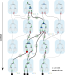
\includegraphics[width=0.8\textwidth]{illustrations/cell-lines}
\end{center}
\caption{\label{fig-cell-lines}
Cellular inheritance of a single chromosome in a diploid population.
Individuals (blue) contain diploid cells (white circles enclosing a homologous pair of chromosomes).
For clarity, only two rounds of mitotic germ-line cell division are shown per individual, and
meiosis is not illustrated in detail.
Lines show prospective inheritance paths for all chromosomes. Solid lines show all possible
retrospective ancestry paths for four chosen chromosomes (indicated by square black ``sampling events'')
sampled from 3 diploid individuals ($D_1$, $D_2$, $D_3$) in the current generation.
Ancestral recombination events and coalescence events are shown as red and blue squares respectively.
The ARG paths for the lower arm of the sampled chromosomes (green) is highlighted as a
think solid line and involves a single recombination event and four coalescence events
(highlighted as deep red and blue squares within individuals $D_5$, $D_{10}$, and $D_{13}$).
ARG lineages also show gametic genomes, contained within shaded circles.
As in Fig.~\ref{fig-arg-in-pedigree}A, inherited regions within the sampled chromosome arm are
shaded by the number of descendant samples.
}
\end{figure}

At the base of this concept is a subtle and important point about which genomes are represented by gARG nodes.
In principle, we can interpret nodes as representing genomes
at any point in the life cycle, for instance, \citet{hudson1983properties} views nodes as representing gametes,
whereas in Fig.~\ref{fig-arg-in-pedigree}A, we present them as genomes within a diploid individual.
In reality, however, recombination and replication of DNA occur at a cellular level,
and respectively correspond to the processes of meiosis and mitosis. Therefore, a comprehensive gARG would not
trace genetic inheritance between diploid individuals, but between cells during the
life cycle of these individuals. This is illustrated in Fig.~\ref{fig-cell-lines}, where we show a simplified
schematic of cellular inheritance in a diploid population over four partially overlapping generations.
In this figure, thick black lines trace an ARG that describes the ancestry of the lower arm of the
four sampled chromosomes. The ``events'' underlying the ARG are shown as red and blue squares,
and the potential ARG nodes are shown as green chromosomal regions. Note that a number of these nodes are
``pass-through'' nodes with one parent and one child, which would normally be omitted.

The unusual feature of this particular example is that three ARG lineages coalesce in one historical individual,
$D_{10}$, whose three children all happen to be ancestors of the sampled chromosomes.
We can see that the process that generates these three child lineages actually consists of two successive bifurcations:
necessitated by the fact that the only known method of reproducing DNA is by (semi-conservative) duplication.
However, if we take each node in the ARG to represents the generalised genome of an individual (rather than the specific
genome of a cell within an individual) we end up representing this as a instantaneous trifucation or polytomy.

There is biological significance to this cellular-level inheritance process. Were a mutation to occur
during the first cell division of $D_{10}$, the two gametes produced by the cells
in the left half of $D_{10}$ could share a mutation not present in the right hand gamete. In other words,
the relationship between three (or more) gametes that originate, without recombination, from the same parental
chromosomes will nevertheless be strictly bifurcating; two of the gametes have a closer relationship with the
third more distant. Of course, unless mutations occur between successive rounds of cell division, the between-cell
relationships will be impossible to infer from the data.

% As with concatenating multiple recombination events, the gARG representation allows us to concatenate within-individual
% coalescence events such that we are not obliged to represent precisely the underlying cellular process. In humans and
% other multicellular diploids, it seems most intuitive to take the nodes in the gARG to represent two haploid genomes within
% a newly fertilised diploid individual. If this individual has 3 or more children, and these children feature in the
% eventual ancestry of the samples, the gARG approach outlined in this paper means that they can be legitimately represented
% by a polytomy in the local trees.

\clearpage
\section{Data encoding of the genome ARG}
\label{sec-gARG-data}

\begin{table}[ht]
    \caption{\label{tab-gARG-data}
    Data encoding of the genome ARG shown in Fig.~\ref{fig-arg-in-pedigree} with the
	node table on the left (having node and time columns) and the edge table on the
	right (having child, parent, and intervals columns).
    }
    \begin{center}
        \begin{tabular}{c|ccc|c|c}
			\multicolumn{2}{c}{Node table}& ~ &\multicolumn{3}{c}{Edge table}\\
			\cline{1-2} \cline{4-6}
            Node & Time & ~ & Child & Parent & Intervals\\
            \cline{1-2} \cline{4-6}
            $\noderef{a}$ & 0 & ~ & $\noderef{a}$ & $\noderef{e}$ & $\{[0,2)\}$\\
            $\noderef{b}$ & 0 & ~ & $\noderef{a}$ & $\noderef{f}$ & $\{[2,10)\}$\\
            $\noderef{c}$ & 0 & ~ & $\noderef{b}$ & $\noderef{g}$ & $\{[0,10)\}$\\
            $\noderef{d}$ & 0 & ~ & $\noderef{c}$ & $\noderef{f}$ & $\{[0,7)\}$\\
            $\noderef{e}$ & 1 & ~ & $\noderef{c}$ & $\noderef{e}$ & $\{[7,10)\}$\\
            $\noderef{f}$ & 1 & ~ & $\noderef{d}$ & $\noderef{h}$ & $\{[0,10)\}$\\
            $\noderef{g}$ & 1 & ~ & $\noderef{e}$ & $\noderef{i}$ & $\{[0,10)\}$\\
            $\noderef{i}$ & 1 & ~ & $\noderef{f}$ & $\noderef{k}$ & $\{[0,10)\}$\\
            $\noderef{k}$ & 2 & ~ & $\noderef{g}$ & $\noderef{i}$ & $\{[0,10)\}$\\
            $\noderef{n}$ & 3 & ~ & $\noderef{h}$ & $\noderef{k}$ & $\{[0,10)\}$\\
            \multicolumn{2}{c}{~}& ~ & $\noderef{i}$ & $\noderef{n}$ & $\{[0,10)\}$\\
            \multicolumn{2}{c}{~}& ~ & $\noderef{k}$ & $\noderef{n}$ & $\{[0,10)\}$
        \end{tabular}
    \end{center}
\end{table}

\clearpage
\section{TODO}
\label{sec-x}

% TODO: we don't seem to cite this figure at all!?

\begin{figure}[ht]
	\begin{center}
		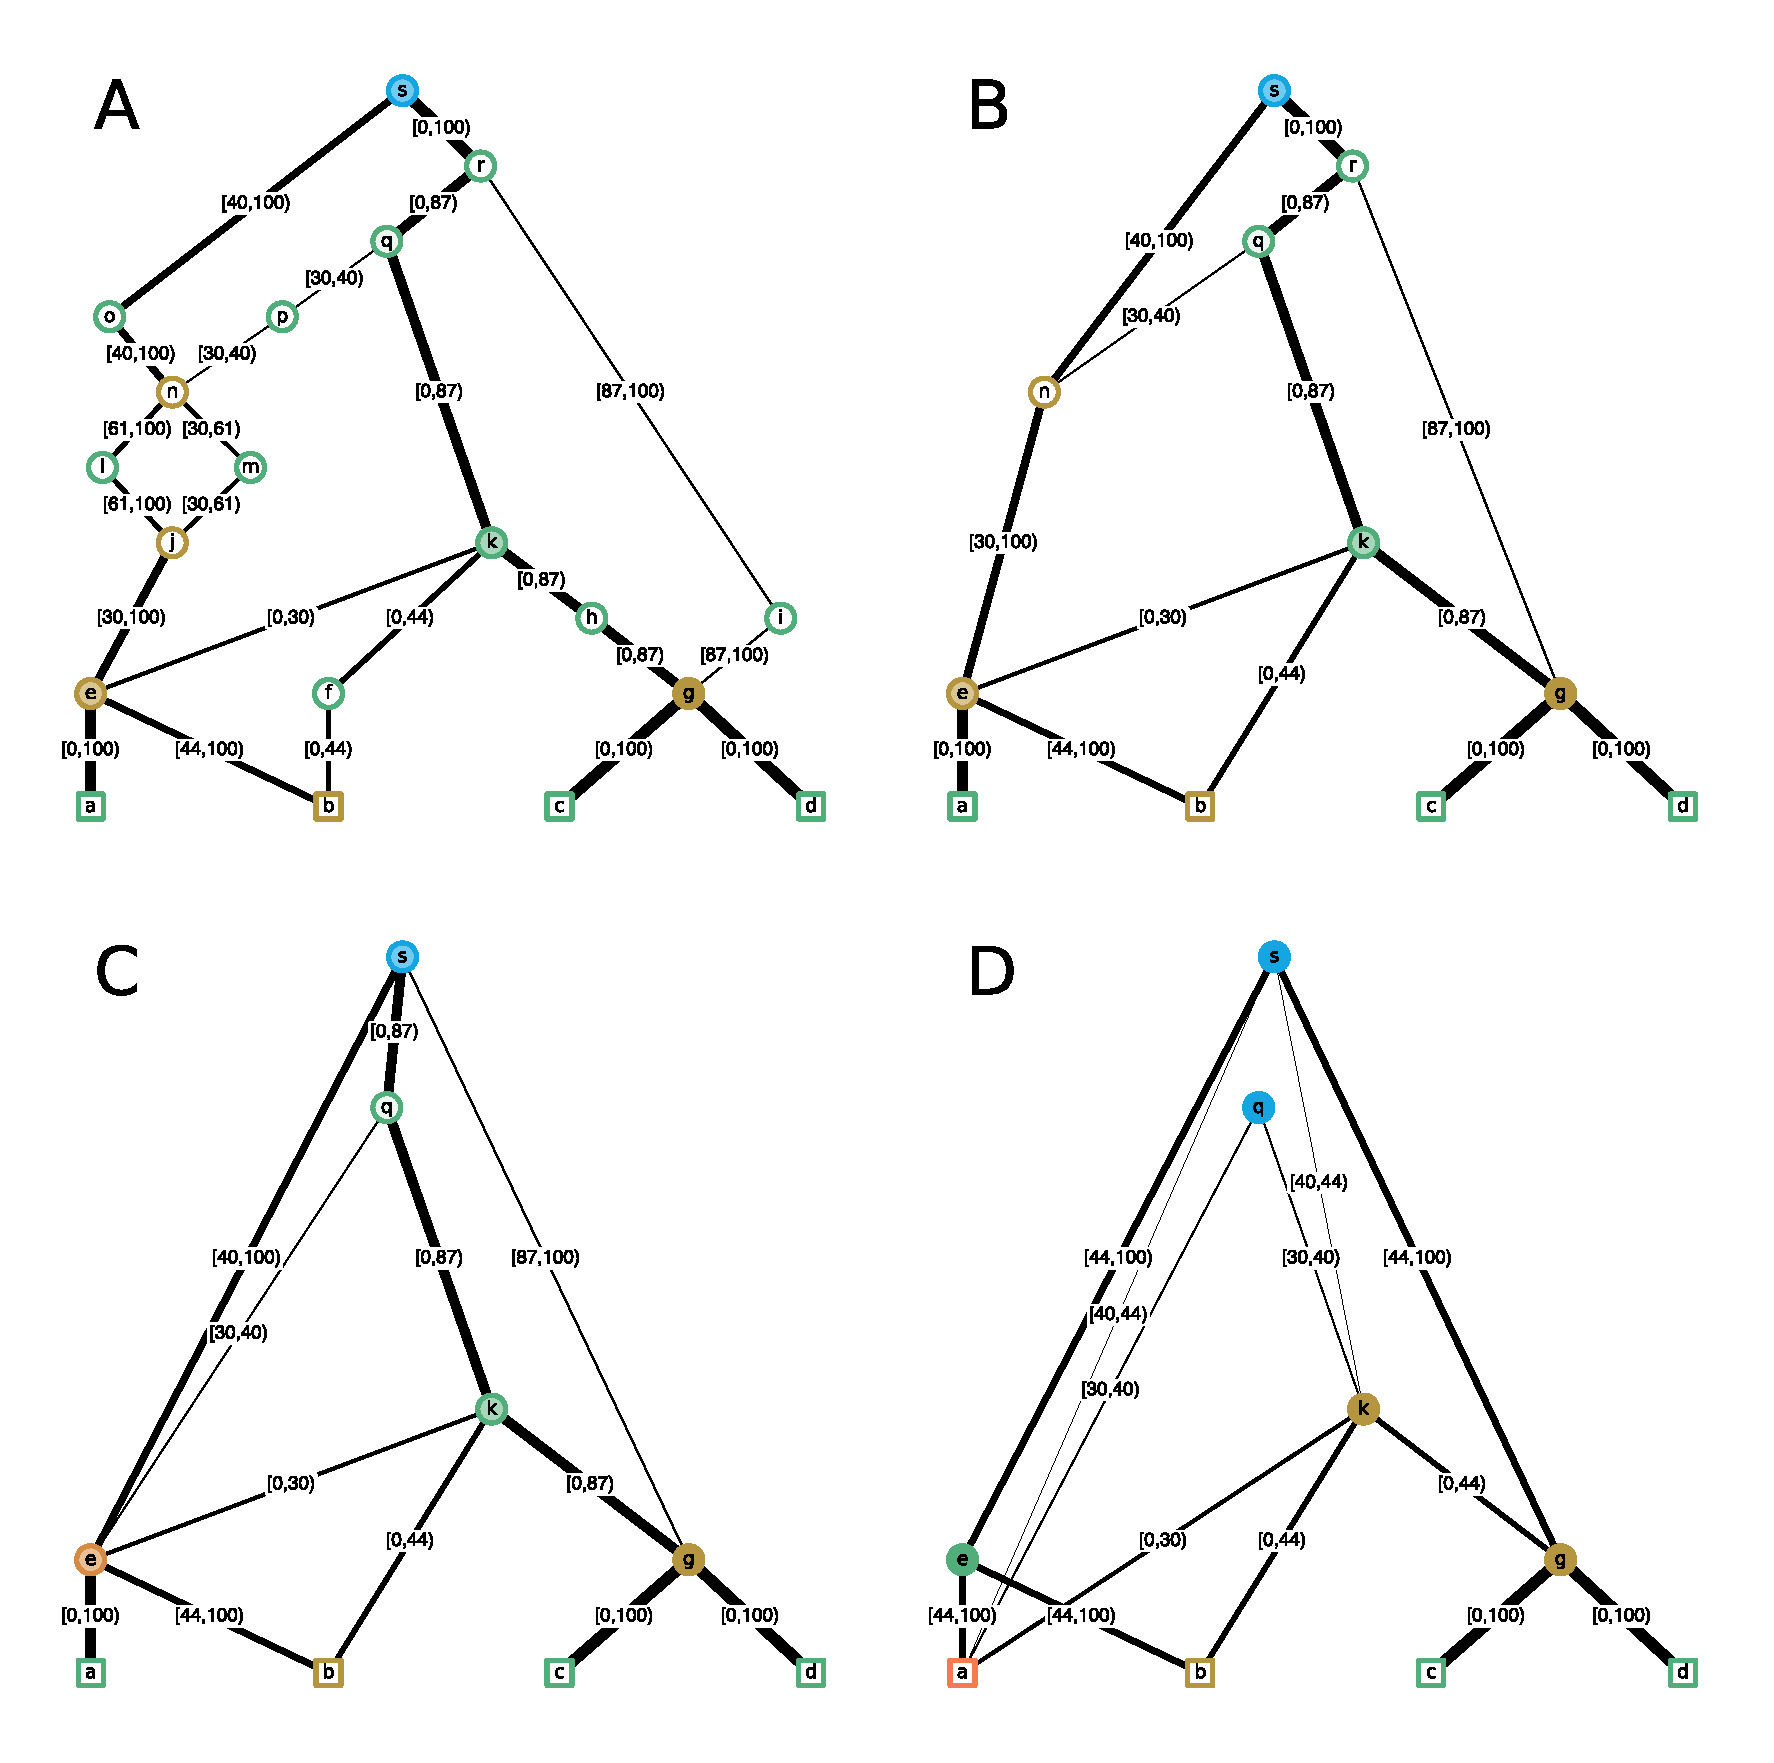
\includegraphics[width=0.8\textwidth]{illustrations/simplification-with-edges.pdf}
	\end{center}
	\caption{\label{fig-simplification-with-edges}
	The four levels of ARG simplification from Fig.~\ref{fig-simplification}A--D, with edge intervals shown.
	}
\end{figure}

\end{document}
